% Options for packages loaded elsewhere
\PassOptionsToPackage{unicode}{hyperref}
\PassOptionsToPackage{hyphens}{url}
%
\documentclass[
]{book}
\usepackage{amsmath,amssymb}
\usepackage{lmodern}
\usepackage{iftex}
\ifPDFTeX
  \usepackage[T1]{fontenc}
  \usepackage[utf8]{inputenc}
  \usepackage{textcomp} % provide euro and other symbols
\else % if luatex or xetex
  \usepackage{unicode-math}
  \defaultfontfeatures{Scale=MatchLowercase}
  \defaultfontfeatures[\rmfamily]{Ligatures=TeX,Scale=1}
\fi
% Use upquote if available, for straight quotes in verbatim environments
\IfFileExists{upquote.sty}{\usepackage{upquote}}{}
\IfFileExists{microtype.sty}{% use microtype if available
  \usepackage[]{microtype}
  \UseMicrotypeSet[protrusion]{basicmath} % disable protrusion for tt fonts
}{}
\makeatletter
\@ifundefined{KOMAClassName}{% if non-KOMA class
  \IfFileExists{parskip.sty}{%
    \usepackage{parskip}
  }{% else
    \setlength{\parindent}{0pt}
    \setlength{\parskip}{6pt plus 2pt minus 1pt}}
}{% if KOMA class
  \KOMAoptions{parskip=half}}
\makeatother
\usepackage{xcolor}
\usepackage{color}
\usepackage{fancyvrb}
\newcommand{\VerbBar}{|}
\newcommand{\VERB}{\Verb[commandchars=\\\{\}]}
\DefineVerbatimEnvironment{Highlighting}{Verbatim}{commandchars=\\\{\}}
% Add ',fontsize=\small' for more characters per line
\usepackage{framed}
\definecolor{shadecolor}{RGB}{248,248,248}
\newenvironment{Shaded}{\begin{snugshade}}{\end{snugshade}}
\newcommand{\AlertTok}[1]{\textcolor[rgb]{0.94,0.16,0.16}{#1}}
\newcommand{\AnnotationTok}[1]{\textcolor[rgb]{0.56,0.35,0.01}{\textbf{\textit{#1}}}}
\newcommand{\AttributeTok}[1]{\textcolor[rgb]{0.77,0.63,0.00}{#1}}
\newcommand{\BaseNTok}[1]{\textcolor[rgb]{0.00,0.00,0.81}{#1}}
\newcommand{\BuiltInTok}[1]{#1}
\newcommand{\CharTok}[1]{\textcolor[rgb]{0.31,0.60,0.02}{#1}}
\newcommand{\CommentTok}[1]{\textcolor[rgb]{0.56,0.35,0.01}{\textit{#1}}}
\newcommand{\CommentVarTok}[1]{\textcolor[rgb]{0.56,0.35,0.01}{\textbf{\textit{#1}}}}
\newcommand{\ConstantTok}[1]{\textcolor[rgb]{0.00,0.00,0.00}{#1}}
\newcommand{\ControlFlowTok}[1]{\textcolor[rgb]{0.13,0.29,0.53}{\textbf{#1}}}
\newcommand{\DataTypeTok}[1]{\textcolor[rgb]{0.13,0.29,0.53}{#1}}
\newcommand{\DecValTok}[1]{\textcolor[rgb]{0.00,0.00,0.81}{#1}}
\newcommand{\DocumentationTok}[1]{\textcolor[rgb]{0.56,0.35,0.01}{\textbf{\textit{#1}}}}
\newcommand{\ErrorTok}[1]{\textcolor[rgb]{0.64,0.00,0.00}{\textbf{#1}}}
\newcommand{\ExtensionTok}[1]{#1}
\newcommand{\FloatTok}[1]{\textcolor[rgb]{0.00,0.00,0.81}{#1}}
\newcommand{\FunctionTok}[1]{\textcolor[rgb]{0.00,0.00,0.00}{#1}}
\newcommand{\ImportTok}[1]{#1}
\newcommand{\InformationTok}[1]{\textcolor[rgb]{0.56,0.35,0.01}{\textbf{\textit{#1}}}}
\newcommand{\KeywordTok}[1]{\textcolor[rgb]{0.13,0.29,0.53}{\textbf{#1}}}
\newcommand{\NormalTok}[1]{#1}
\newcommand{\OperatorTok}[1]{\textcolor[rgb]{0.81,0.36,0.00}{\textbf{#1}}}
\newcommand{\OtherTok}[1]{\textcolor[rgb]{0.56,0.35,0.01}{#1}}
\newcommand{\PreprocessorTok}[1]{\textcolor[rgb]{0.56,0.35,0.01}{\textit{#1}}}
\newcommand{\RegionMarkerTok}[1]{#1}
\newcommand{\SpecialCharTok}[1]{\textcolor[rgb]{0.00,0.00,0.00}{#1}}
\newcommand{\SpecialStringTok}[1]{\textcolor[rgb]{0.31,0.60,0.02}{#1}}
\newcommand{\StringTok}[1]{\textcolor[rgb]{0.31,0.60,0.02}{#1}}
\newcommand{\VariableTok}[1]{\textcolor[rgb]{0.00,0.00,0.00}{#1}}
\newcommand{\VerbatimStringTok}[1]{\textcolor[rgb]{0.31,0.60,0.02}{#1}}
\newcommand{\WarningTok}[1]{\textcolor[rgb]{0.56,0.35,0.01}{\textbf{\textit{#1}}}}
\usepackage{longtable,booktabs,array}
\usepackage{calc} % for calculating minipage widths
% Correct order of tables after \paragraph or \subparagraph
\usepackage{etoolbox}
\makeatletter
\patchcmd\longtable{\par}{\if@noskipsec\mbox{}\fi\par}{}{}
\makeatother
% Allow footnotes in longtable head/foot
\IfFileExists{footnotehyper.sty}{\usepackage{footnotehyper}}{\usepackage{footnote}}
\makesavenoteenv{longtable}
\usepackage{graphicx}
\makeatletter
\def\maxwidth{\ifdim\Gin@nat@width>\linewidth\linewidth\else\Gin@nat@width\fi}
\def\maxheight{\ifdim\Gin@nat@height>\textheight\textheight\else\Gin@nat@height\fi}
\makeatother
% Scale images if necessary, so that they will not overflow the page
% margins by default, and it is still possible to overwrite the defaults
% using explicit options in \includegraphics[width, height, ...]{}
\setkeys{Gin}{width=\maxwidth,height=\maxheight,keepaspectratio}
% Set default figure placement to htbp
\makeatletter
\def\fps@figure{htbp}
\makeatother
\setlength{\emergencystretch}{3em} % prevent overfull lines
\providecommand{\tightlist}{%
  \setlength{\itemsep}{0pt}\setlength{\parskip}{0pt}}
\setcounter{secnumdepth}{5}
\usepackage{booktabs}
\ifLuaTeX
  \usepackage{selnolig}  % disable illegal ligatures
\fi
\usepackage[]{natbib}
\bibliographystyle{plainnat}
\IfFileExists{bookmark.sty}{\usepackage{bookmark}}{\usepackage{hyperref}}
\IfFileExists{xurl.sty}{\usepackage{xurl}}{} % add URL line breaks if available
\urlstyle{same} % disable monospaced font for URLs
\hypersetup{
  pdftitle={Introduction à R},
  pdfauthor={Thomas Denecker \& Stevenn Volant},
  hidelinks,
  pdfcreator={LaTeX via pandoc}}

\title{Introduction à R}
\author{Thomas Denecker \& Stevenn Volant}
\date{2022-11-15}

\begin{document}
\maketitle

{
\setcounter{tocdepth}{1}
\tableofcontents
}
\hypertarget{pruxe9sentation-du-cours}{%
\chapter{Présentation du cours}\label{pruxe9sentation-du-cours}}

Bienvenues dans le cour Introduction à R de l'EBAII ! Pour accompagner ce cours, Thomas Denecker et Stevenn Volant vous proposent ce livre. C'est une grande première alors n'hésitez pas à nous faire des retours.

\hypertarget{a-propos-de-du-livre}{%
\section{A propos de du livre}\label{a-propos-de-du-livre}}

L'objectif de ce livre est d'accompagné les apprenants de l'école EBAII.

\hypertarget{demandez-le-programme}{%
\section{Demandez le programme}\label{demandez-le-programme}}

\begin{longtable}[]{@{}llll@{}}
\toprule()
Debut & Fin & Durée & Lieu \\
\midrule()
\endhead
8:30 & 10:15 & 01:45 & HDF \\
\bottomrule()
\end{longtable}

\hypertarget{intervenants}{%
\section{Intervenants}\label{intervenants}}

\begin{itemize}
\tightlist
\item
  Thomas Denecker -- \href{mailto:thomas.denecker@france-bioinformatique.fr}{\nolinkurl{thomas.denecker@france-bioinformatique.fr}}
\item
  Stevenn Volant - \href{mailto:stevenn.volant@pasteur.fr}{\nolinkurl{stevenn.volant@pasteur.fr}}
\end{itemize}

La version ``slides'' a été créée initialement par Hugo Varet -- \href{mailto:hugo.varet@pasteur.fr}{\nolinkurl{hugo.varet@pasteur.fr}}

\hypertarget{r-en-quelques-mots}{%
\chapter{R en quelques mots}\label{r-en-quelques-mots}}

\hypertarget{pourquoi}{%
\section{Pourquoi ?}\label{pourquoi}}

Langage de programmation qui permet de :
- manipuler des données : importer, transformer, exporter faire des analyses statistiques plus ou moins complexes : description, exploration, modélisation\ldots{}
- créer des (jolies) figures

\hypertarget{comment-lavoir}{%
\section{Comment l'avoir ?}\label{comment-lavoir}}

Disponible sur \href{https://cran.r-project.org/}{RCRAN}

\hypertarget{sur-quel-os}{%
\section{Sur quel OS ?}\label{sur-quel-os}}

Tous !

\hypertarget{historique}{%
\section{Historique}\label{historique}}

\begin{itemize}
\tightlist
\item
  1993 : Début du projet R
\item
  2000 : sortie de R 1.0.0
\item
  2022 : R 4.2.2
\end{itemize}

\hypertarget{r-vs-excel}{%
\section{R vs Excel}\label{r-vs-excel}}

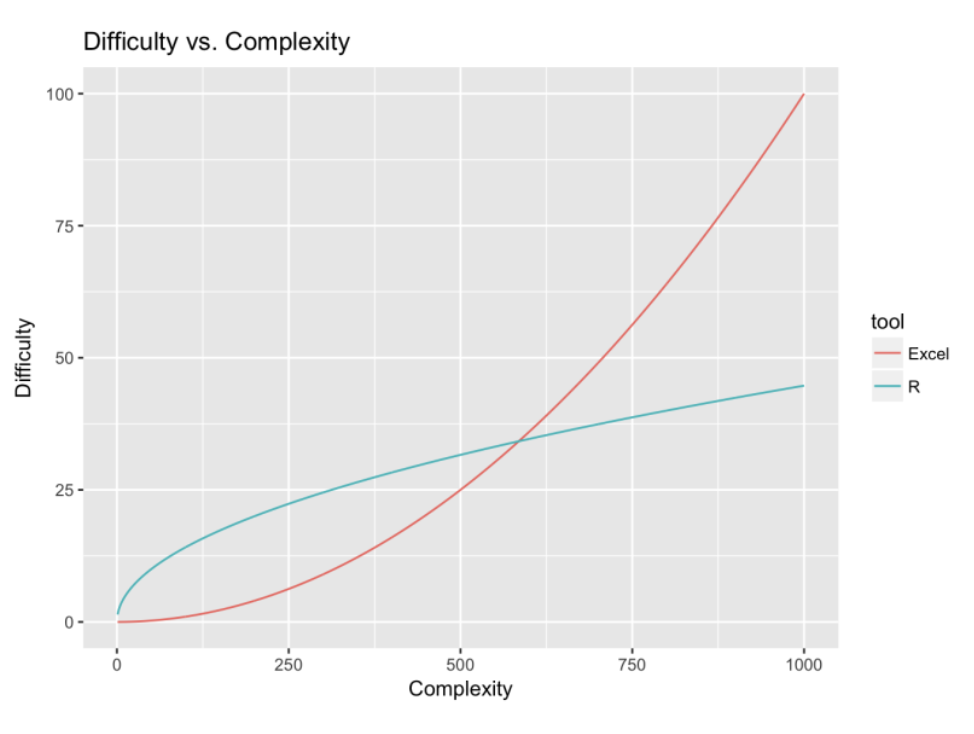
\includegraphics{images/rblogger.png}
Source: R-bloggers

\hypertarget{pourquoi-plus-excel}{%
\subsection{Pourquoi plus Excel ?}\label{pourquoi-plus-excel}}

Un exemple parmi tant d'autres !

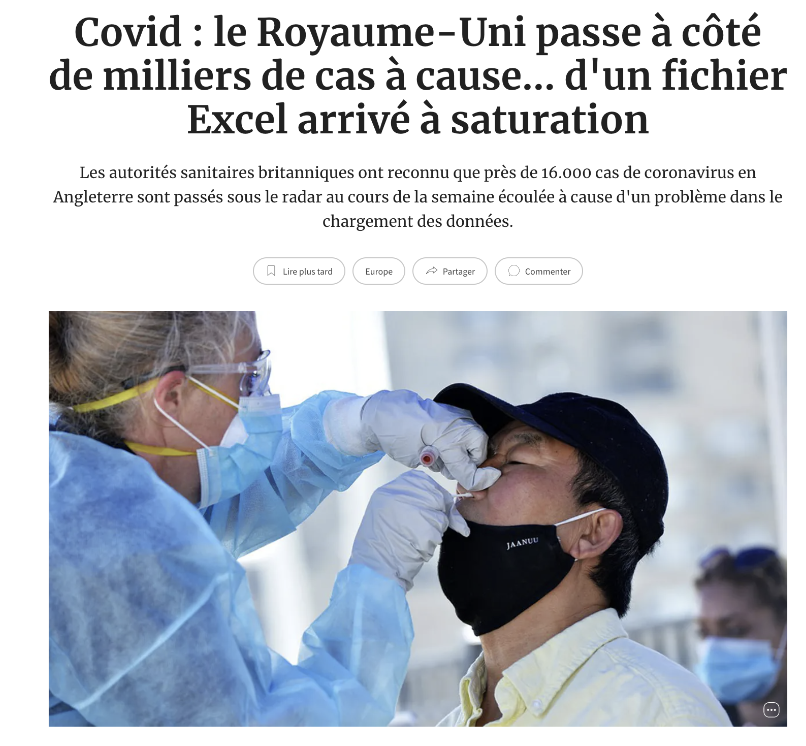
\includegraphics{images/covid.png}

Source Alexandre Counis, Les Echos, 5 oct. 2020

\hypertarget{avantages-et-inconvuxe9nients}{%
\section{Avantages et inconvénients}\label{avantages-et-inconvuxe9nients}}

\hypertarget{avantages}{%
\subsection{Avantages}\label{avantages}}

\begin{itemize}
\tightlist
\item
  Souplesse d'utilisation pour réaliser des analyses statistiques
\item
  Libre et gratuit, même s'il existe maintenant des versions payantes de RStudio (shiny et/ou server)
\item
  Reproductibilité des analyses en écrivant/sauvegardant les commandes R dans des scripts
\item
  Large communauté d'utilisateurs/aide en ligne
\item
  Grand nombre de packages spécifiques
\end{itemize}

\hypertarget{inconvuxe9nients}{%
\subsection{Inconvénients}\label{inconvuxe9nients}}

\hypertarget{geeks-and-repetitive-tasks}{%
\section{Geeks and repetitive tasks}\label{geeks-and-repetitive-tasks}}

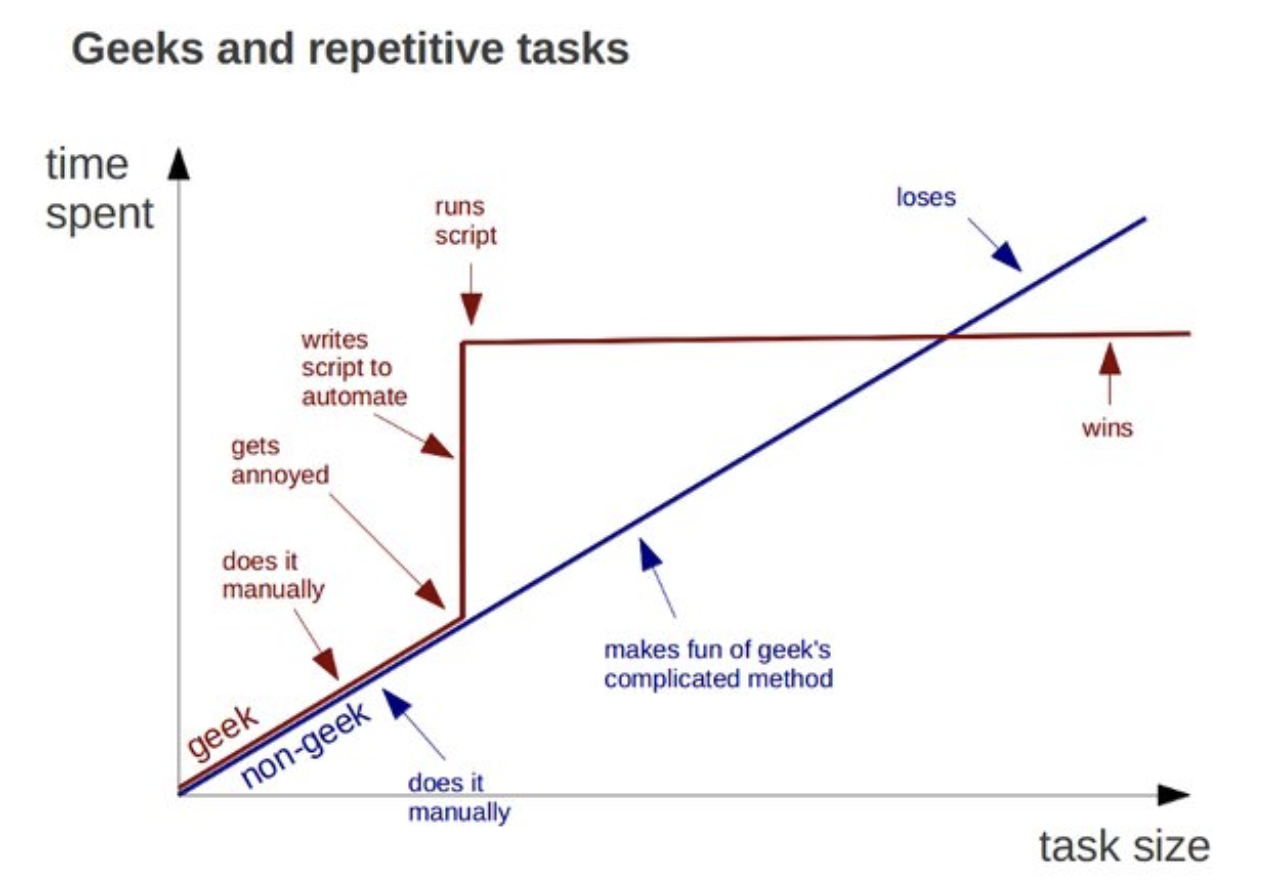
\includegraphics{images/geeks.png}

\hypertarget{r-sait-tout-faire}{%
\section{R sait tout faire}\label{r-sait-tout-faire}}

Lire un tableau de données

\begin{Shaded}
\begin{Highlighting}[]
\FunctionTok{read.table}\NormalTok{()}
\end{Highlighting}
\end{Shaded}

Fusionner deux tableaux

\begin{Shaded}
\begin{Highlighting}[]
\FunctionTok{merge}\NormalTok{()}
\end{Highlighting}
\end{Shaded}

Filtrer des lignes

\begin{Shaded}
\begin{Highlighting}[]
\NormalTok{data[data}\SpecialCharTok{$}\NormalTok{x }\SpecialCharTok{\textgreater{}} \DecValTok{10}\NormalTok{]}
\end{Highlighting}
\end{Shaded}

Sélectionner des colonnes

\begin{Shaded}
\begin{Highlighting}[]
\NormalTok{data[,}\FunctionTok{c}\NormalTok{(“x”,”y”)]}
\end{Highlighting}
\end{Shaded}

Rechercher une chaîne de caractères

\begin{Shaded}
\begin{Highlighting}[]
\FunctionTok{grep}\NormalTok{()}
\end{Highlighting}
\end{Shaded}

Réaliser une ACP

\begin{Shaded}
\begin{Highlighting}[]
\FunctionTok{prcomp}\NormalTok{()}
\end{Highlighting}
\end{Shaded}

Calculer une moyenne

\begin{Shaded}
\begin{Highlighting}[]
\FunctionTok{mean}\NormalTok{()}
\end{Highlighting}
\end{Shaded}

Additionner deux matrices

\begin{Shaded}
\begin{Highlighting}[]
\NormalTok{mat1 }\SpecialCharTok{+}\NormalTok{ mat2}
\end{Highlighting}
\end{Shaded}

Exporter un tableau de données

\begin{Shaded}
\begin{Highlighting}[]
\FunctionTok{write.table}\NormalTok{()}
\end{Highlighting}
\end{Shaded}

Calculer une variance

\begin{Shaded}
\begin{Highlighting}[]
\FunctionTok{var}\NormalTok{()}
\end{Highlighting}
\end{Shaded}

Régression linéaire

\begin{Shaded}
\begin{Highlighting}[]
\FunctionTok{lm}\NormalTok{()}
\end{Highlighting}
\end{Shaded}

Tracer une courbe

\begin{Shaded}
\begin{Highlighting}[]
\FunctionTok{plot}\NormalTok{()}
\end{Highlighting}
\end{Shaded}

Tester une hypothèse

\begin{Shaded}
\begin{Highlighting}[]
\FunctionTok{t.test}\NormalTok{()}
\end{Highlighting}
\end{Shaded}

Dessiner un histogramme

\begin{Shaded}
\begin{Highlighting}[]
\FunctionTok{hist}\NormalTok{()}
\end{Highlighting}
\end{Shaded}

Convertir des données

\begin{Shaded}
\begin{Highlighting}[]
\FunctionTok{as.matrix}\NormalTok{()}
\end{Highlighting}
\end{Shaded}

\hypertarget{comment-utiliser-r}{%
\chapter{Comment utiliser R ?}\label{comment-utiliser-r}}

\hypertarget{modes-dutilisation-liste-non-exhaustive}{%
\section{Modes d'utilisation (liste non exhaustive)}\label{modes-dutilisation-liste-non-exhaustive}}

\begin{itemize}
\tightlist
\item
  Localement via le terminal
\item
  Localement via RStudio (utilisation classique)
\item
  Sur un serveur via le terminal et une connexion ssh
\item
  Sur un serveur via un navigateur web pour accéder à RStudio server
\item
  Sur un serveur via un navigateur web pour accéder à RStudio server par Jupyter
\end{itemize}

\hypertarget{ouverture-ou-connexion-uxe0-rstudio}{%
\section{Ouverture ou connexion à RStudio}\label{ouverture-ou-connexion-uxe0-rstudio}}

3 alternatives :

\begin{enumerate}
\def\labelenumi{\arabic{enumi}.}
\item
  Ouvrir RStudio sur votre propre ordinateur (si installé)
\item
  Vous connecter au serveur Web RStudio de l'IFB
  \url{https://rstudio.cluster.france-bioinformatique.fr}
  puis vous identifier
\end{enumerate}

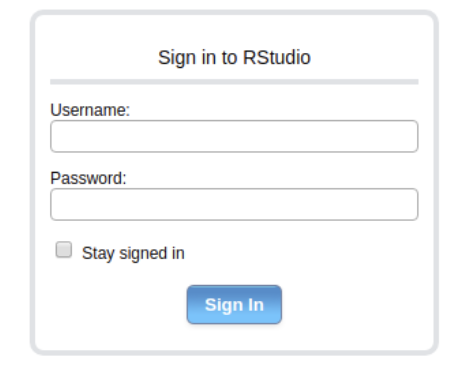
\includegraphics{images/coRstudio.png}

\begin{enumerate}
\def\labelenumi{\arabic{enumi}.}
\setcounter{enumi}{2}
\tightlist
\item
  Vous connecter via Jupyter lab de l'IFB
  \url{https://jupyterhub.cluster.france-bioinformatique.fr}
  puis cliquer sur l'icône RStudio
\end{enumerate}

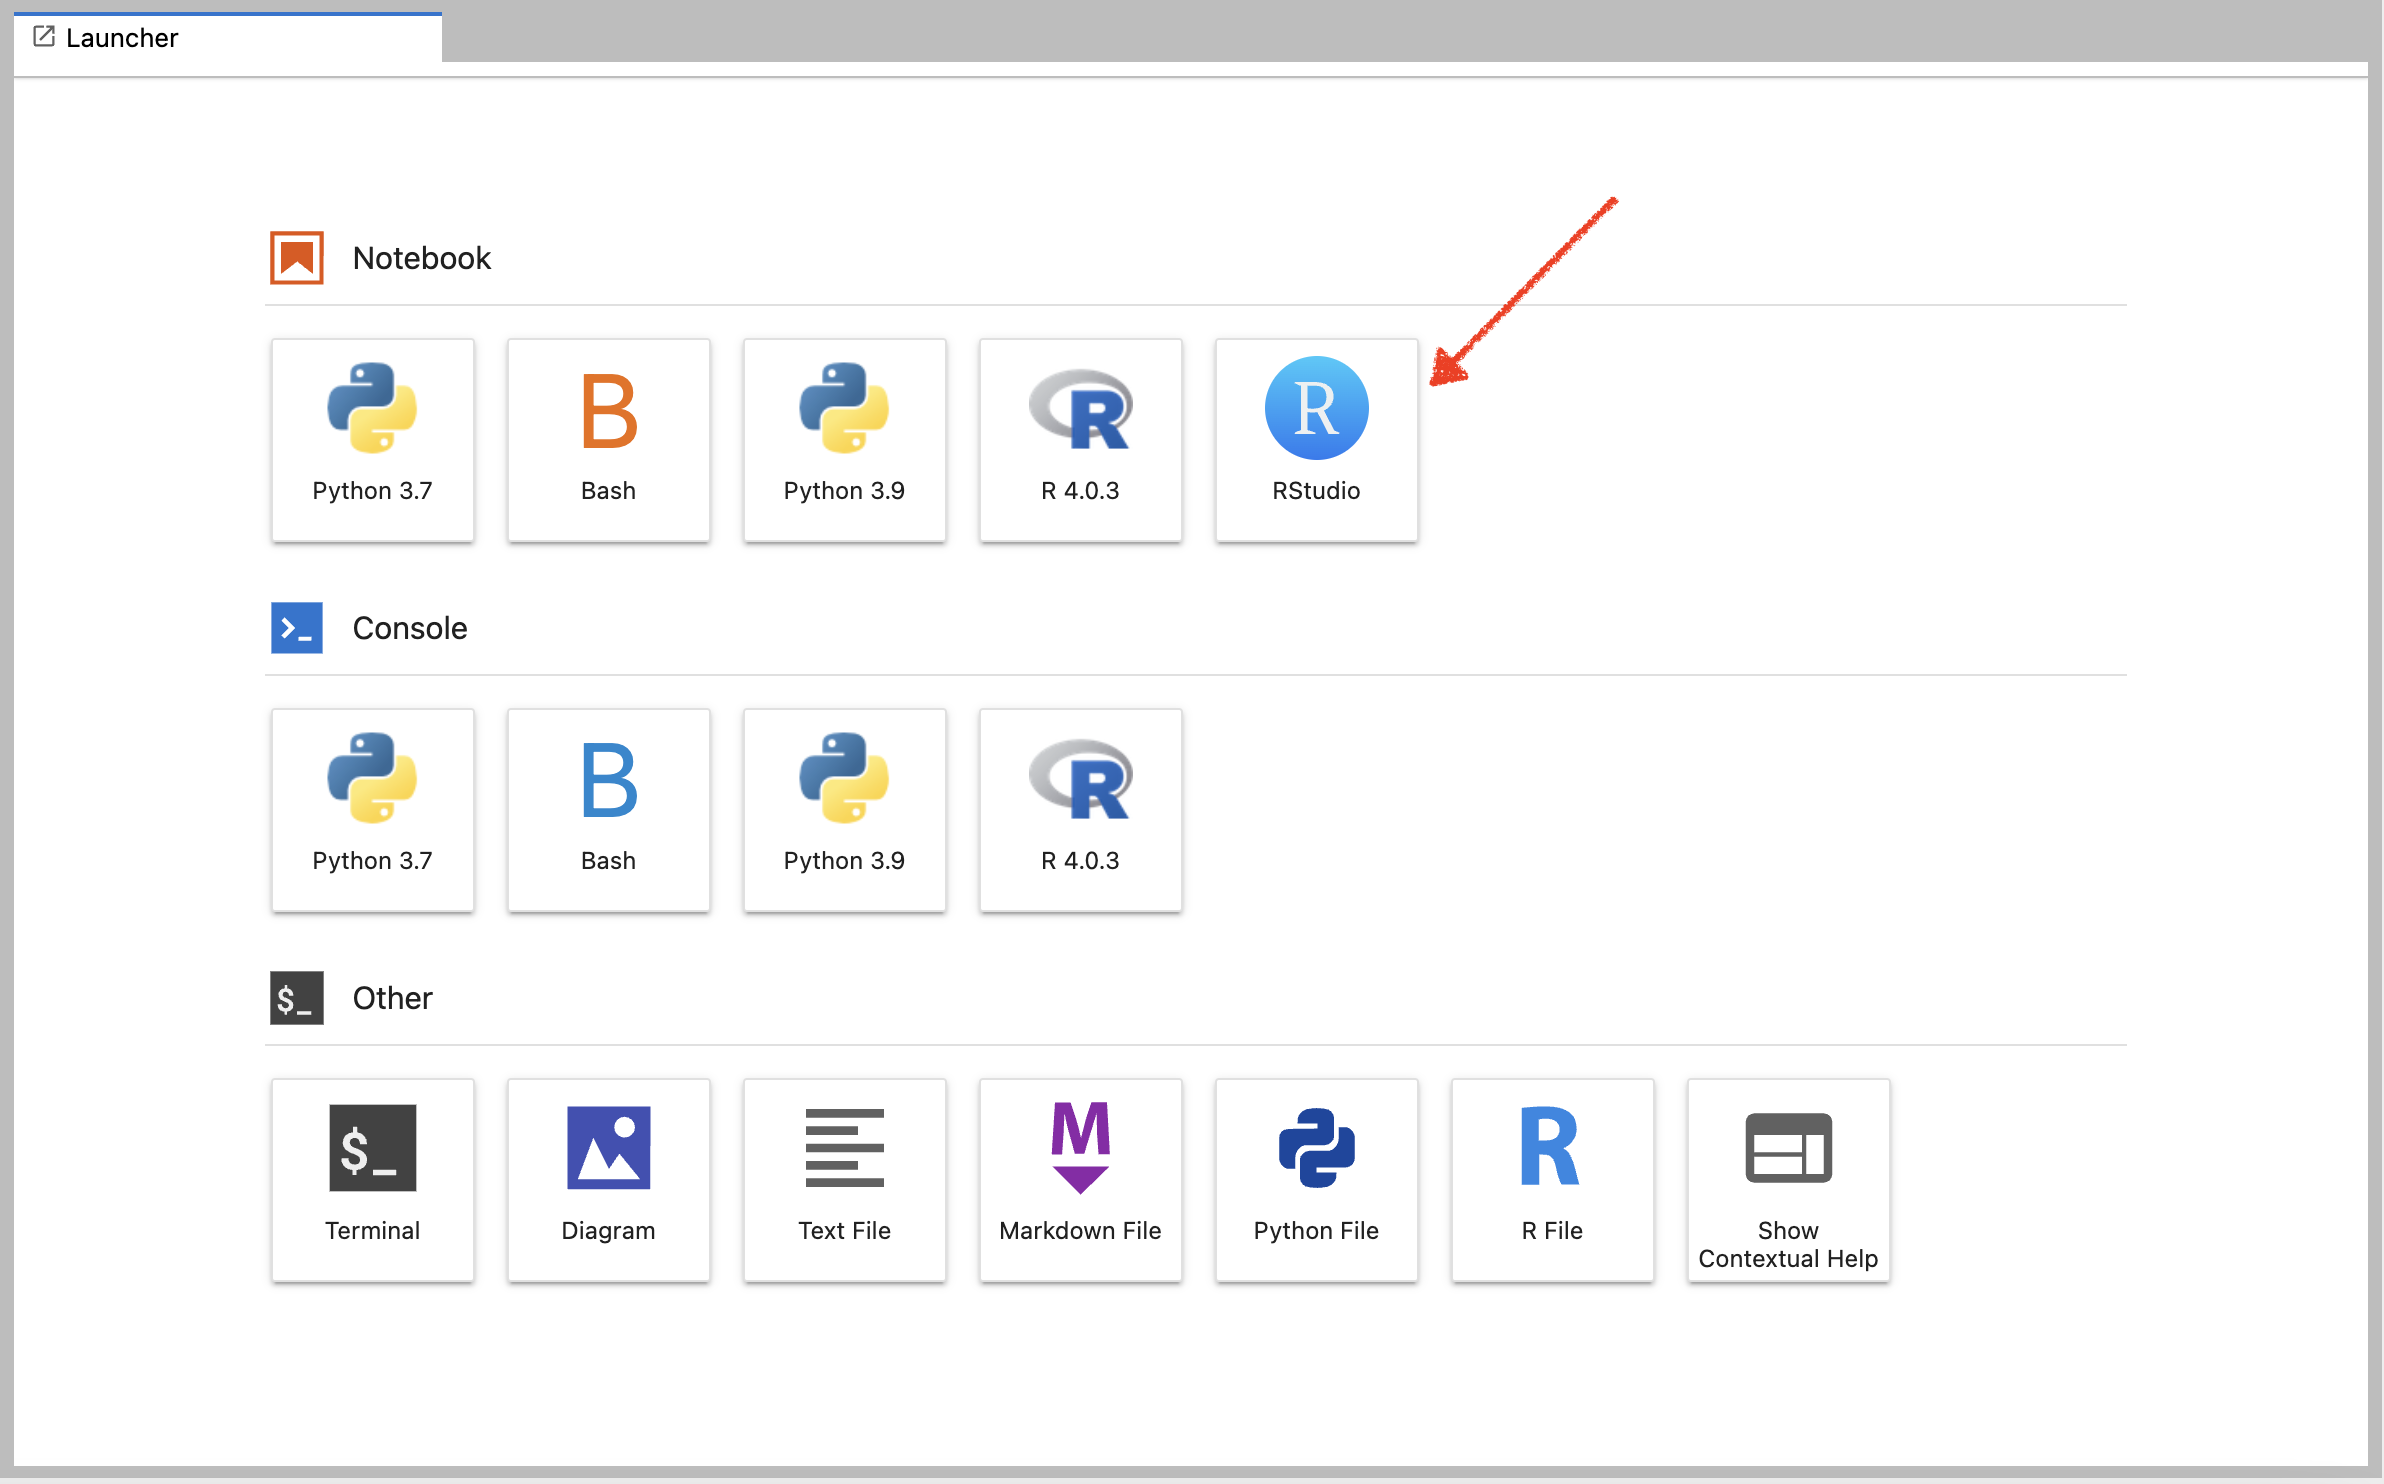
\includegraphics{images/jupyterRstudio.png}

\hypertarget{rstudio}{%
\section{RStudio}\label{rstudio}}

\begin{itemize}
\tightlist
\item
  Disponible depuis 2011
\item
  Logiciel facilitant l'utilisation de R via 4 panneaux
\item
  Chaque panneau présente plusieurs onglets (fonctionnalités complémentaires)
\end{itemize}

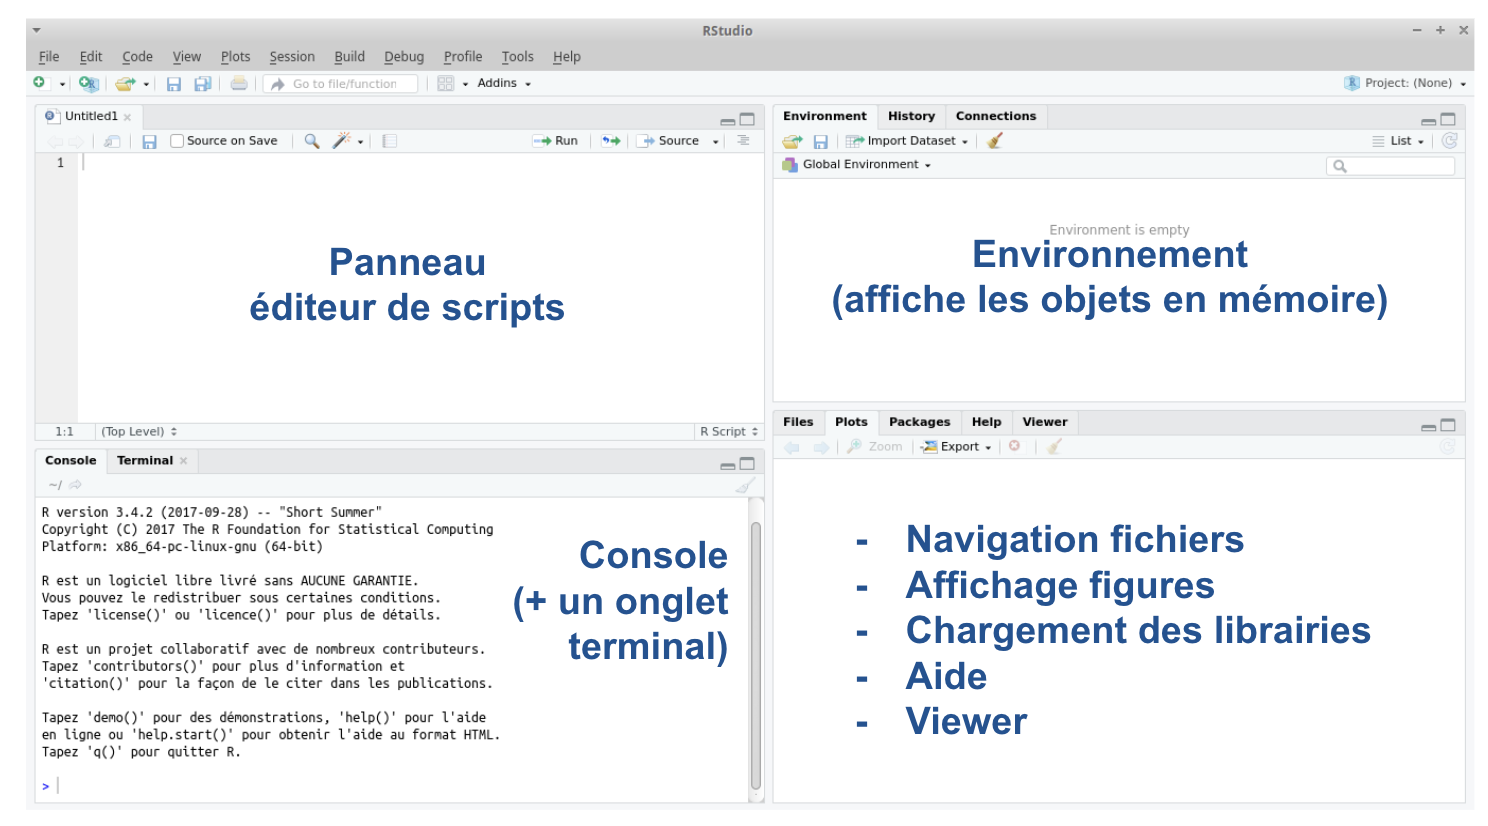
\includegraphics{images/rstudio.png}

\hypertarget{premiers-pas}{%
\chapter{Premiers pas}\label{premiers-pas}}

\hypertarget{r-sait-tout-faire-il-compte}{%
\section{R sait tout faire : il compte !}\label{r-sait-tout-faire-il-compte}}

Tapez les commandes suivantes dans le panneau Console de RStudio

\begin{Shaded}
\begin{Highlighting}[]
\DecValTok{2} \SpecialCharTok{+} \DecValTok{3}
\end{Highlighting}
\end{Shaded}

\begin{verbatim}
## [1] 5
\end{verbatim}

\begin{Shaded}
\begin{Highlighting}[]
\DecValTok{4} \SpecialCharTok{*} \DecValTok{5}
\end{Highlighting}
\end{Shaded}

\begin{verbatim}
## [1] 20
\end{verbatim}

\begin{Shaded}
\begin{Highlighting}[]
\DecValTok{6} \SpecialCharTok{/} \DecValTok{4}
\end{Highlighting}
\end{Shaded}

\begin{verbatim}
## [1] 1.5
\end{verbatim}

\begin{Shaded}
\begin{Highlighting}[]
\DecValTok{1}\SpecialCharTok{:}\DecValTok{10}
\end{Highlighting}
\end{Shaded}

\begin{verbatim}
##  [1]  1  2  3  4  5  6  7  8  9 10
\end{verbatim}

\begin{Shaded}
\begin{Highlighting}[]
\DecValTok{8}\SpecialCharTok{:{-}}\DecValTok{9}
\end{Highlighting}
\end{Shaded}

\begin{verbatim}
##  [1]  8  7  6  5  4  3  2  1  0 -1 -2 -3 -4 -5 -6 -7 -8 -9
\end{verbatim}

\begin{Shaded}
\begin{Highlighting}[]
\DecValTok{1}\NormalTok{,}\DecValTok{2}
\end{Highlighting}
\end{Shaded}

\begin{Shaded}
\begin{Highlighting}[]
\FloatTok{1.2}
\end{Highlighting}
\end{Shaded}

\begin{verbatim}
## [1] 1.2
\end{verbatim}

\hypertarget{notion-de-variableobjet}{%
\section{Notion de variable/objet}\label{notion-de-variableobjet}}

Créer une variable nommée a et lui assigner une valeur

\begin{Shaded}
\begin{Highlighting}[]
\NormalTok{a }\OtherTok{\textless{}{-}} \DecValTok{2}
\end{Highlighting}
\end{Shaded}

Afficher la valeur de la variable a

\begin{Shaded}
\begin{Highlighting}[]
\FunctionTok{print}\NormalTok{(a)}
\end{Highlighting}
\end{Shaded}

\begin{verbatim}
## [1] 2
\end{verbatim}

Même résultat: si on évoque le nom de variable, R l'imprime

\begin{Shaded}
\begin{Highlighting}[]
\NormalTok{a}
\end{Highlighting}
\end{Shaded}

\begin{verbatim}
## [1] 2
\end{verbatim}

Assigner une valeur à une seconde variable

\begin{Shaded}
\begin{Highlighting}[]
\NormalTok{b }\OtherTok{\textless{}{-}} \DecValTok{3}
\end{Highlighting}
\end{Shaded}

Effectuer un calcul avec 2 variables

\begin{Shaded}
\begin{Highlighting}[]
\NormalTok{a\_plus\_b }\OtherTok{\textless{}{-}}\NormalTok{ a }\SpecialCharTok{+}\NormalTok{ b}
\end{Highlighting}
\end{Shaded}

Afficher le contenu de la variable a\_plus\_b

\begin{Shaded}
\begin{Highlighting}[]
\FunctionTok{print}\NormalTok{(a\_plus\_b)}
\end{Highlighting}
\end{Shaded}

\begin{verbatim}
## [1] 5
\end{verbatim}

Changer la valeur de a

\begin{Shaded}
\begin{Highlighting}[]
\NormalTok{a }\OtherTok{\textless{}{-}} \DecValTok{7} 
\end{Highlighting}
\end{Shaded}

Note: le contenu de a\_plus\_b n'est pas modifié

\begin{Shaded}
\begin{Highlighting}[]
\FunctionTok{print}\NormalTok{(a\_plus\_b) }
\end{Highlighting}
\end{Shaded}

\begin{verbatim}
## [1] 5
\end{verbatim}

On recalcule a\_plus\_b

\begin{Shaded}
\begin{Highlighting}[]
\NormalTok{a\_plus\_b }\OtherTok{\textless{}{-}}\NormalTok{ a }\SpecialCharTok{+}\NormalTok{ b }
\end{Highlighting}
\end{Shaded}

La nouvelle valeur tient compte de la modification de a

\begin{Shaded}
\begin{Highlighting}[]
\FunctionTok{print}\NormalTok{(a\_plus\_b)}
\end{Highlighting}
\end{Shaded}

\begin{verbatim}
## [1] 10
\end{verbatim}

Créer un vecteur

\begin{Shaded}
\begin{Highlighting}[]
\NormalTok{vec1 }\OtherTok{\textless{}{-}}  \FunctionTok{c}\NormalTok{(}\DecValTok{1}\NormalTok{,}\DecValTok{10}\NormalTok{)}
\end{Highlighting}
\end{Shaded}

Créer un vecteur contenant une séquence d'entiers de 1 à 10

\begin{Shaded}
\begin{Highlighting}[]
\NormalTok{vec2 }\OtherTok{\textless{}{-}}  \DecValTok{1}\SpecialCharTok{:}\DecValTok{10}
\end{Highlighting}
\end{Shaded}

Somme d'un vecteur et d'un nombre

\begin{Shaded}
\begin{Highlighting}[]
\NormalTok{vec2 }\SpecialCharTok{+}\NormalTok{ a }
\end{Highlighting}
\end{Shaded}

\begin{verbatim}
##  [1]  8  9 10 11 12 13 14 15 16 17
\end{verbatim}

Vecteur de chaînes de caractères

\begin{Shaded}
\begin{Highlighting}[]
\NormalTok{vec3 }\OtherTok{\textless{}{-}}  \FunctionTok{c}\NormalTok{(}\StringTok{"riri"}\NormalTok{, }\StringTok{"fifi"}\NormalTok{, }\StringTok{"loulou"}\NormalTok{)}
\end{Highlighting}
\end{Shaded}

Diviser un vecteur de nombres par un nombre

\begin{Shaded}
\begin{Highlighting}[]
\NormalTok{vec2 }\SpecialCharTok{/} \DecValTok{2}
\end{Highlighting}
\end{Shaded}

\begin{verbatim}
##  [1] 0.5 1.0 1.5 2.0 2.5 3.0 3.5 4.0 4.5 5.0
\end{verbatim}

Diviser des chaînes de caractères par un nombre

\begin{Shaded}
\begin{Highlighting}[]
\NormalTok{vec3  }\SpecialCharTok{/} \DecValTok{2}   
\end{Highlighting}
\end{Shaded}

\textbf{Attention} : Noms de variables interdits: TRUE, FALSE, T, F, c, t, pi, data, LETTERS, letters, \ldots{}

\hypertarget{import-de-donnuxe9es}{%
\chapter{Import de données}\label{import-de-donnuxe9es}}

\hypertarget{version-avec-les-boutons}{%
\section{Version ``Avec les boutons''}\label{version-avec-les-boutons}}

\hypertarget{cruxe9ation-dun-dossier-intro_r-pour-vos-ruxe9sultats-de-ce-tp}{%
\subsection{Création d'un dossier intro\_R pour vos résultats de ce TP}\label{cruxe9ation-dun-dossier-intro_r-pour-vos-ruxe9sultats-de-ce-tp}}

\textbf{Attention} Dans votre espace projet ou votre home.

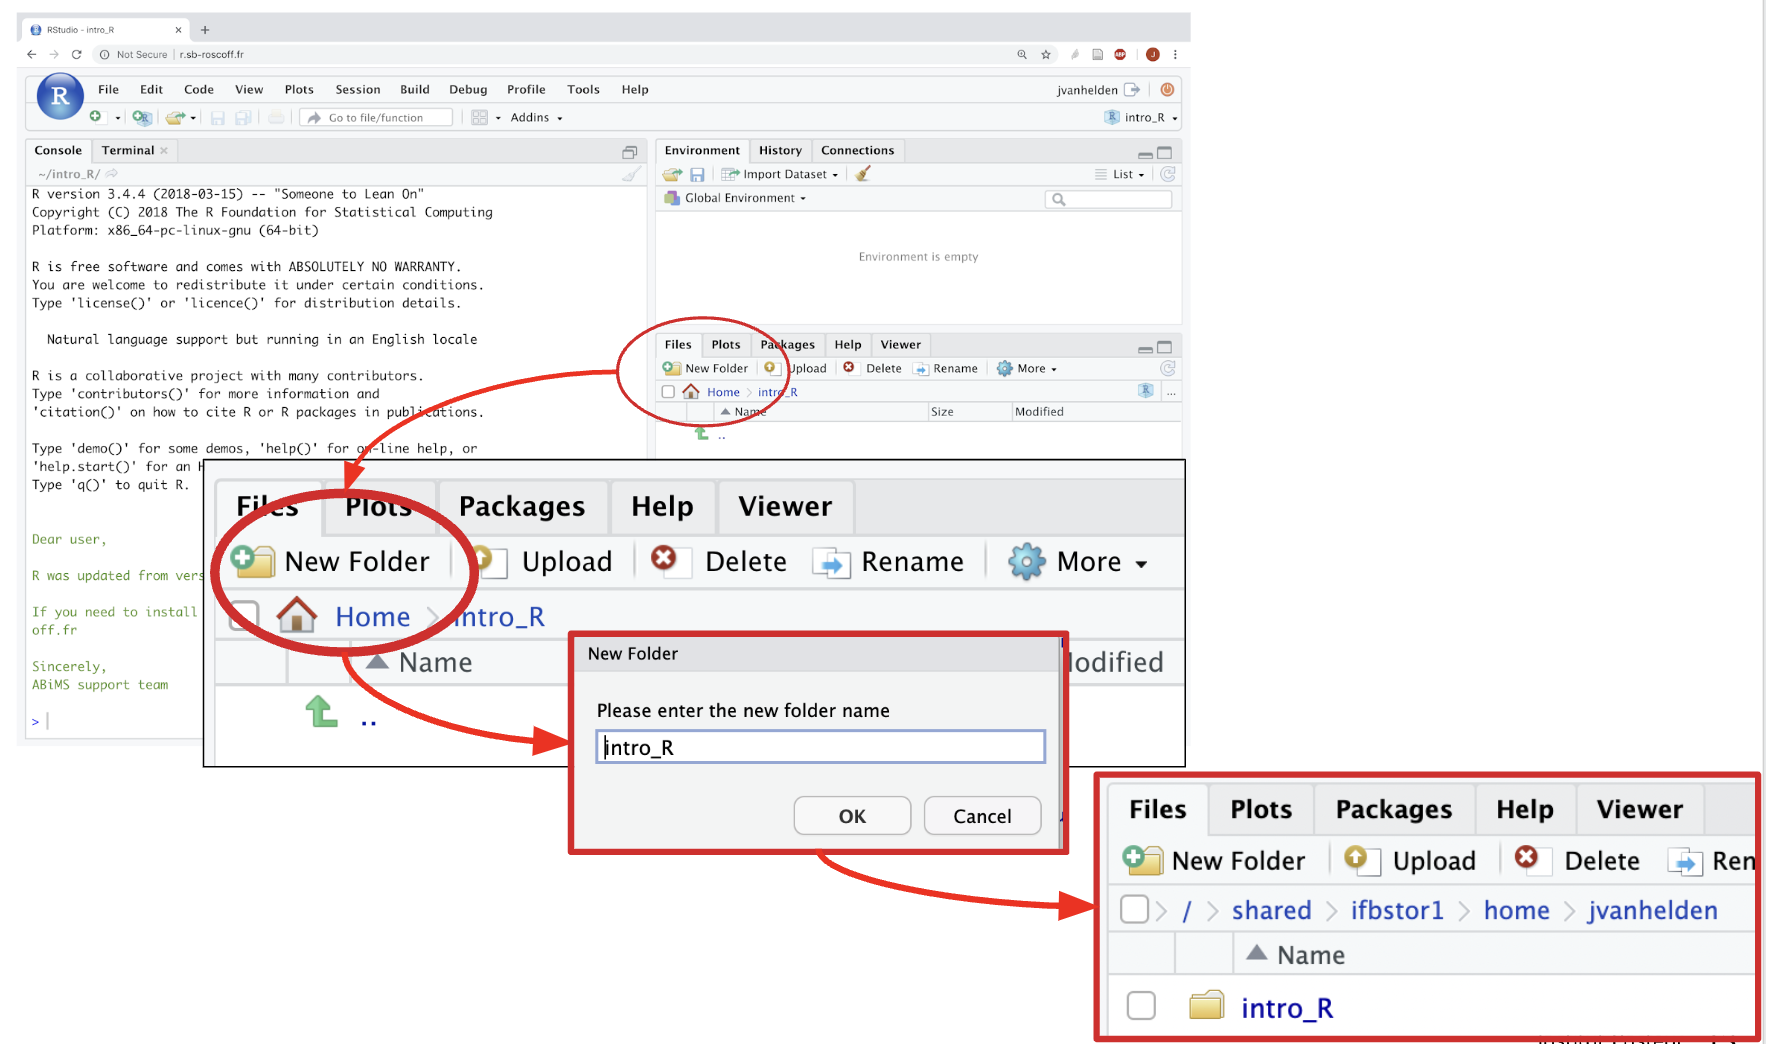
\includegraphics{images/createIntro.png}

\hypertarget{duxe9placement-dans-le-dossier-intro_r}{%
\subsection{Déplacement dans le dossier ``intro\_R''}\label{duxe9placement-dans-le-dossier-intro_r}}

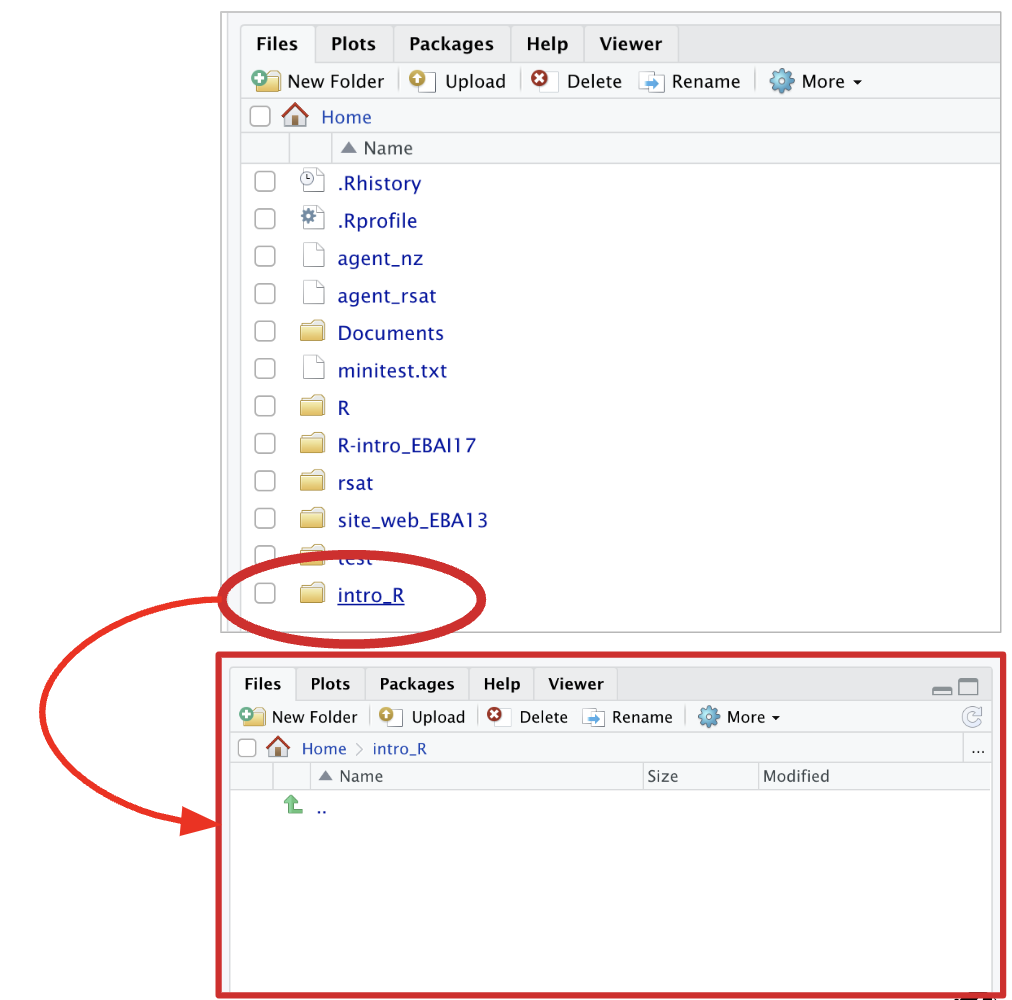
\includegraphics{images/moveIntro.png}

\hypertarget{duxe9finissez-votre-dossier-espace-de-travail-working-directory}{%
\subsection{Définissez votre dossier espace de travail (working directory)}\label{duxe9finissez-votre-dossier-espace-de-travail-working-directory}}

\begin{enumerate}
\def\labelenumi{\arabic{enumi}.}
\tightlist
\item
  Dans le menu ``Session'', lancez ``Choose Directory \ldots{}''
\item
  Naviguez jusqu'à votre dossier intro\_R
\item
  Double-cliquez dessus pour l'ouvrir
\item
  Cliquez Choose
\end{enumerate}

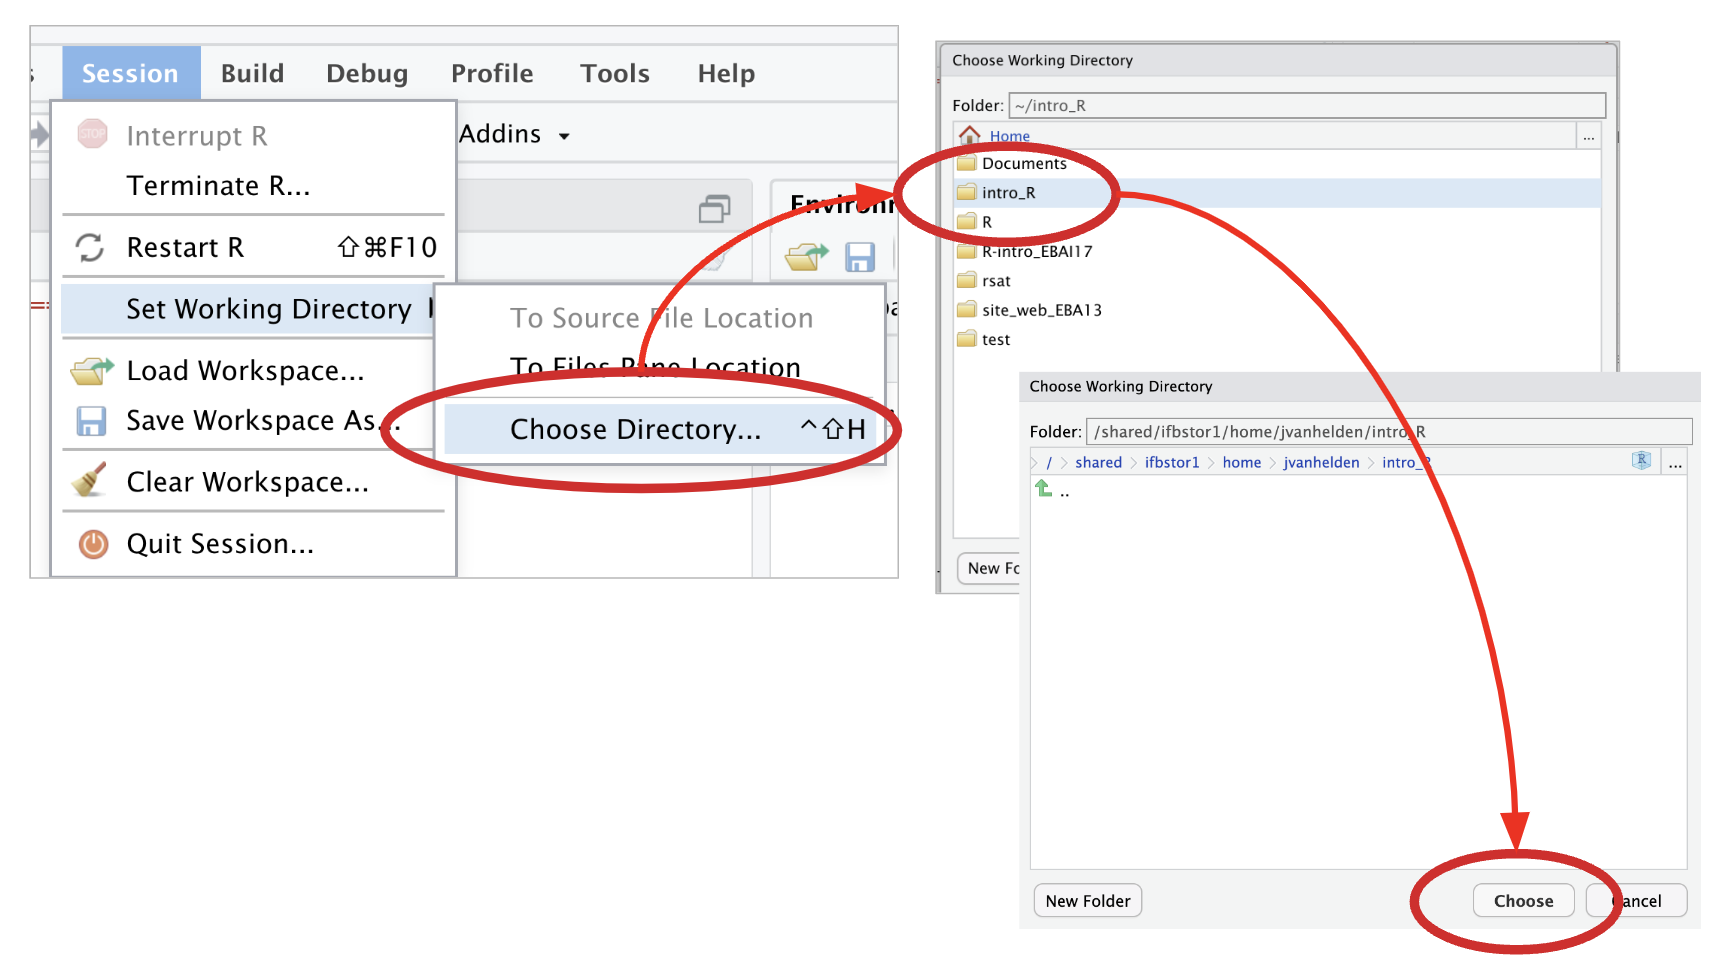
\includegraphics{images/setWd.png}

\hypertarget{tuxe9luxe9chargez-les-fichiers-sur-votre-machine}{%
\subsection{Téléchargez les fichiers sur votre machine}\label{tuxe9luxe9chargez-les-fichiers-sur-votre-machine}}

A partir d'un navigateur Web, téléchargez et enregistrez sur votre ordi les fichiers de données
- \href{https://raw.githubusercontent.com/IFB-ElixirFr/EBAII/master/2022/ebaiin1/intro_R/expression.txt}{expression.txt}: données d'expressions pour 4 échantillons
- \href{https://raw.githubusercontent.com/IFB-ElixirFr/EBAII/master/2022/ebaiin1/intro_R/annotation.csv}{annotation.csv}: informations sur les gènes (id, name, chr, start, stop)

Attention: veillez à sauvegarder les fichiers
- sous leur nom original,
- avec les extensions .txt et .csv respectives (certains navigateurs omettent l'extension, ce qui poserait problème pour la suite du TP)

\hypertarget{tuxe9luxe9versement-upload-des-donnuxe9es}{%
\subsection{Téléversement (``upload'') des données}\label{tuxe9luxe9versement-upload-des-donnuxe9es}}

Au moyen du bouton ``Upload'', téléversez les fichiers d'expression et d'annotation depuis votre ordinateur vers votre compte sur le serveur.

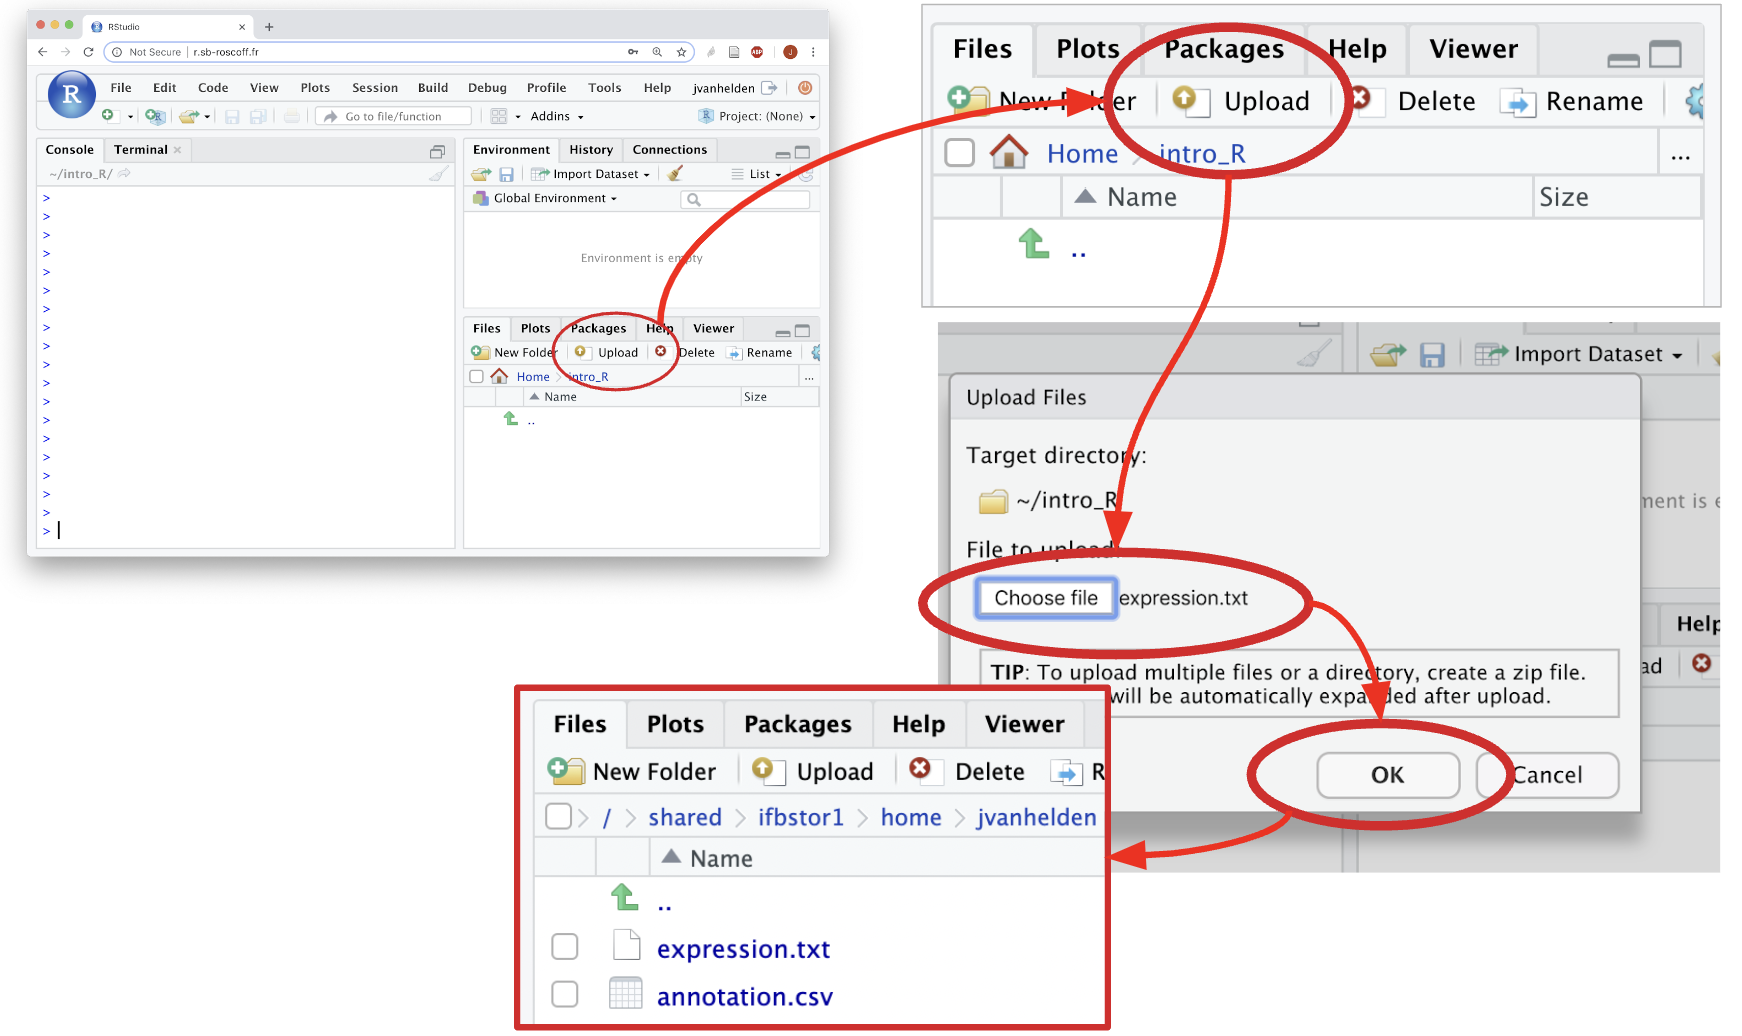
\includegraphics{images/uploadData.png}

\hypertarget{on-efface-tout-et-on-recommence}{%
\subsection{On efface tout et on recommence}\label{on-efface-tout-et-on-recommence}}

\begin{enumerate}
\def\labelenumi{\arabic{enumi}.}
\tightlist
\item
  Sélectionnez les deux fichiers
\item
  Effacez-les sans pitié
\end{enumerate}

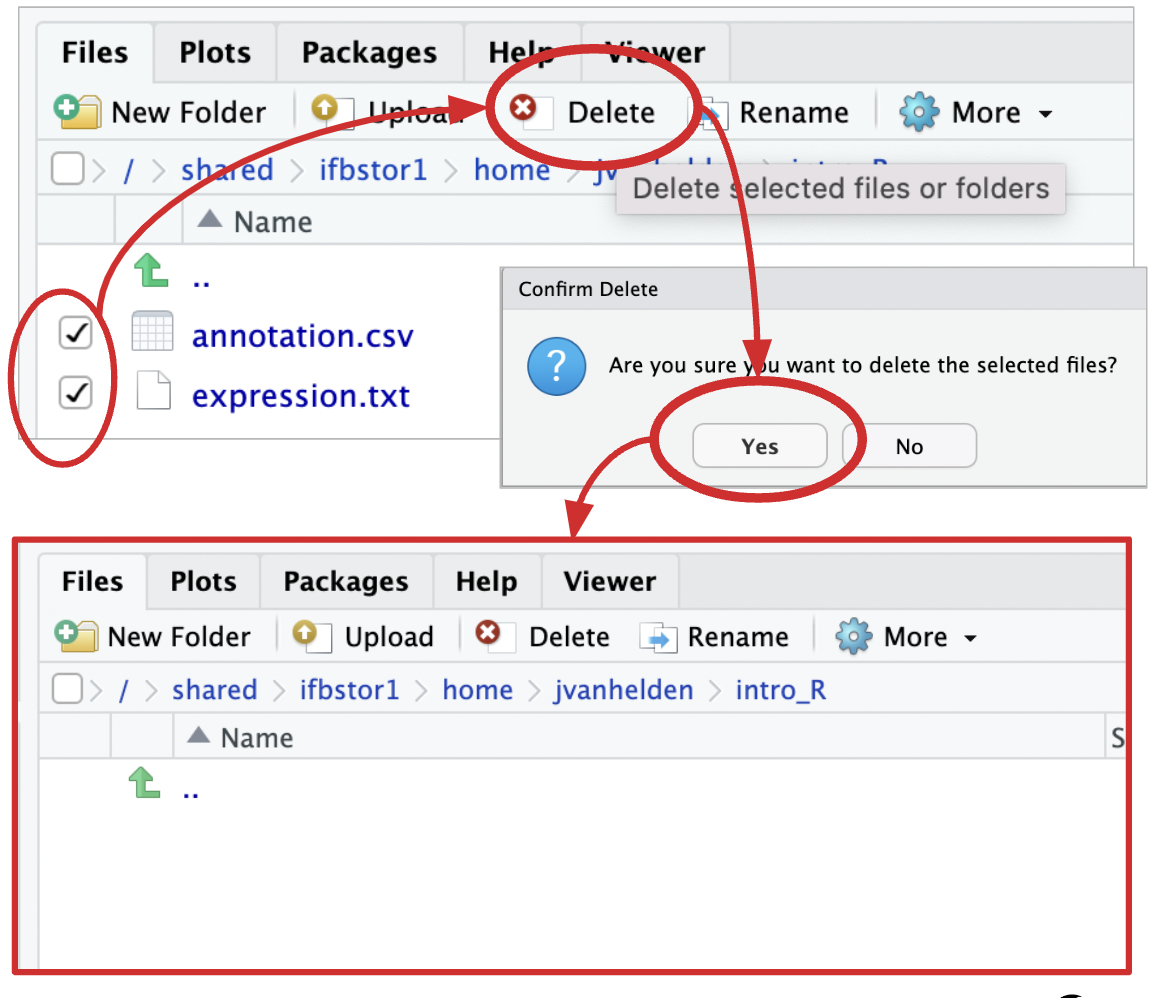
\includegraphics{images/delete.png}

(nous allons vous montrer deux autres façons de les téléverser)

\hypertarget{the-r-geek-way-v2-directement-depuis-rstudio}{%
\section{The ``R geek'' way (V2, directement depuis Rstudio)}\label{the-r-geek-way-v2-directement-depuis-rstudio}}

Attention ! Dans votre espace projet !

\hypertarget{creation-de-larborescence}{%
\subsection{Creation de l'arborescence}\label{creation-de-larborescence}}

Aller dans \textbf{votre} espace projet !

Dans tous les commandes ci-dessous, remplacer toujours \texttt{form\_2022\_32/EBAII\_IntroR} par votre nom d'espace projet

Note : Pour les personnes ne travaillant pas sur le cluster mais par exemple en local, vous pouvez sans soucis remplacer l'adresse par une adresse sur votre ordinateur.

\begin{Shaded}
\begin{Highlighting}[]
\FunctionTok{setwd}\NormalTok{(}\StringTok{"/shared/ifbstor1/projects/form\_2022\_32/EBAII\_IntroR"}\NormalTok{)}
\end{Highlighting}
\end{Shaded}

Définir une variable qui indique le chemin du dossier de travail (working directory).

\begin{Shaded}
\begin{Highlighting}[]
\NormalTok{my\_work\_dir }\OtherTok{\textless{}{-}} \StringTok{"/shared/ifbstor1/projects/form\_2022\_32/EBAII\_IntroR/intro\_R"} 
\end{Highlighting}
\end{Shaded}

S'il n'existe pas encore, créer le dossier de travail. (Commande Unix équivalente: \texttt{mkdir\ -p\ /shared/ifbstor1/projects/form\_2022\_32/EBAII\_IntroR/intro\_R})

\begin{Shaded}
\begin{Highlighting}[]
\FunctionTok{dir.create}\NormalTok{(my\_work\_dir, }\AttributeTok{recursive =} \ConstantTok{TRUE}\NormalTok{, }\AttributeTok{showWarnings =} \ConstantTok{FALSE}\NormalTok{)}
\end{Highlighting}
\end{Shaded}

Où suis-je ? (Commande Unix équivalente: \texttt{pwd})

\begin{Shaded}
\begin{Highlighting}[]
\FunctionTok{getwd}\NormalTok{()}
\end{Highlighting}
\end{Shaded}

\begin{verbatim}
## [1] "/shared/ifbstor1/projects/form_2022_32/EBAII_IntroR"
\end{verbatim}

Aller dans ce dossier de travail (Commande Unix équivalente: \texttt{cd\ /shared/ifbstor1/projects/form\_2022\_32/EBAII\_IntroR/intro\_R})

\begin{Shaded}
\begin{Highlighting}[]
\FunctionTok{setwd}\NormalTok{(my\_work\_dir)}
\end{Highlighting}
\end{Shaded}

Et maintenant, où suis-je ?

\begin{Shaded}
\begin{Highlighting}[]
\FunctionTok{getwd}\NormalTok{()}
\end{Highlighting}
\end{Shaded}

\begin{verbatim}
## [1] "/shared/ifbstor1/projects/form_2022_32/EBAII_IntroR"
\end{verbatim}

Qu'y a-t-il par ici ? (Commande Unix équivalente: \texttt{ls})

\begin{Shaded}
\begin{Highlighting}[]
\FunctionTok{list.files}\NormalTok{()}
\end{Highlighting}
\end{Shaded}

\begin{verbatim}
##  [1] "_bookdown_files"    "_bookdown.yml"      "_main_files"       
##  [4] "_main.Rmd"          "_output.yml"        "01-intro.Rmd"      
##  [7] "02-how.Rmd"         "03-firstSteps.Rmd"  "04-uploadData.Rmd" 
## [10] "05-readData.Rmd"    "06-manipulate.Rmd"  "07-references.Rmd" 
## [13] "annotation.csv"     "book.bib"           "docs"              
## [16] "EBAII_IntroR.Rproj" "expression.txt"     "images"            
## [19] "index.Rmd"          "intro_R"            "LICENSE"           
## [22] "packages.bib"       "preamble.tex"       "README.md"         
## [25] "style.css"
\end{verbatim}

Un autre nom pour la même commande

\begin{Shaded}
\begin{Highlighting}[]
\FunctionTok{dir}\NormalTok{()}
\end{Highlighting}
\end{Shaded}

\begin{verbatim}
##  [1] "_bookdown_files"    "_bookdown.yml"      "_main_files"       
##  [4] "_main.Rmd"          "_output.yml"        "01-intro.Rmd"      
##  [7] "02-how.Rmd"         "03-firstSteps.Rmd"  "04-uploadData.Rmd" 
## [10] "05-readData.Rmd"    "06-manipulate.Rmd"  "07-references.Rmd" 
## [13] "annotation.csv"     "book.bib"           "docs"              
## [16] "EBAII_IntroR.Rproj" "expression.txt"     "images"            
## [19] "index.Rmd"          "intro_R"            "LICENSE"           
## [22] "packages.bib"       "preamble.tex"       "README.md"         
## [25] "style.css"
\end{verbatim}

\hypertarget{tuxe9luxe9charger-un-fichier}{%
\subsection{Télécharger un fichier}\label{tuxe9luxe9charger-un-fichier}}

Nous avons montré ci-dessus comment télécharger des fichiers en utilisant l'interface graphique de RStudio.

Alternativement, on peut télécharger des fichiers au moyen de la commande R download.file.

Les deux commandes suivantes permettent de télécharger les fichiers utilisés pour les exercices.

\begin{Shaded}
\begin{Highlighting}[]
\FunctionTok{download.file}\NormalTok{(}\AttributeTok{url =} \StringTok{"https://raw.githubusercontent.com/IFB{-}ElixirFr/EBAII/master/2022/ebaiin1/intro\_R/expression.txt"}\NormalTok{, }\AttributeTok{destfile =} \StringTok{"expression.txt"}\NormalTok{)}
\end{Highlighting}
\end{Shaded}

\begin{Shaded}
\begin{Highlighting}[]
\FunctionTok{download.file}\NormalTok{(}\AttributeTok{url =} \StringTok{"https://raw.githubusercontent.com/IFB{-}ElixirFr/EBAII/master/2022/ebaiin1/intro\_R/annotation.csv"}\NormalTok{, }\AttributeTok{destfile =} \StringTok{"annotation.csv"}\NormalTok{)}
\end{Highlighting}
\end{Shaded}

Note : équivalent de la commande \texttt{wget} sous Unix.

Qu'y a-t-il par ici ? (Commande Unix équivalente: \texttt{ls})

\begin{Shaded}
\begin{Highlighting}[]
\FunctionTok{list.files}\NormalTok{()}
\end{Highlighting}
\end{Shaded}

\begin{verbatim}
##  [1] "_bookdown_files"    "_bookdown.yml"      "_main_files"       
##  [4] "_main.Rmd"          "_output.yml"        "01-intro.Rmd"      
##  [7] "02-how.Rmd"         "03-firstSteps.Rmd"  "04-uploadData.Rmd" 
## [10] "05-readData.Rmd"    "06-manipulate.Rmd"  "07-references.Rmd" 
## [13] "annotation.csv"     "book.bib"           "docs"              
## [16] "EBAII_IntroR.Rproj" "expression.txt"     "images"            
## [19] "index.Rmd"          "intro_R"            "LICENSE"           
## [22] "packages.bib"       "preamble.tex"       "README.md"         
## [25] "style.css"
\end{verbatim}

\hypertarget{on-efface-tout-et-on-recommence-1}{%
\subsection{On efface tout et on recommence}\label{on-efface-tout-et-on-recommence-1}}

\begin{enumerate}
\def\labelenumi{\arabic{enumi}.}
\tightlist
\item
  Sélectionnez les deux fichiers
\item
  Effacez-les sans pitié
\end{enumerate}

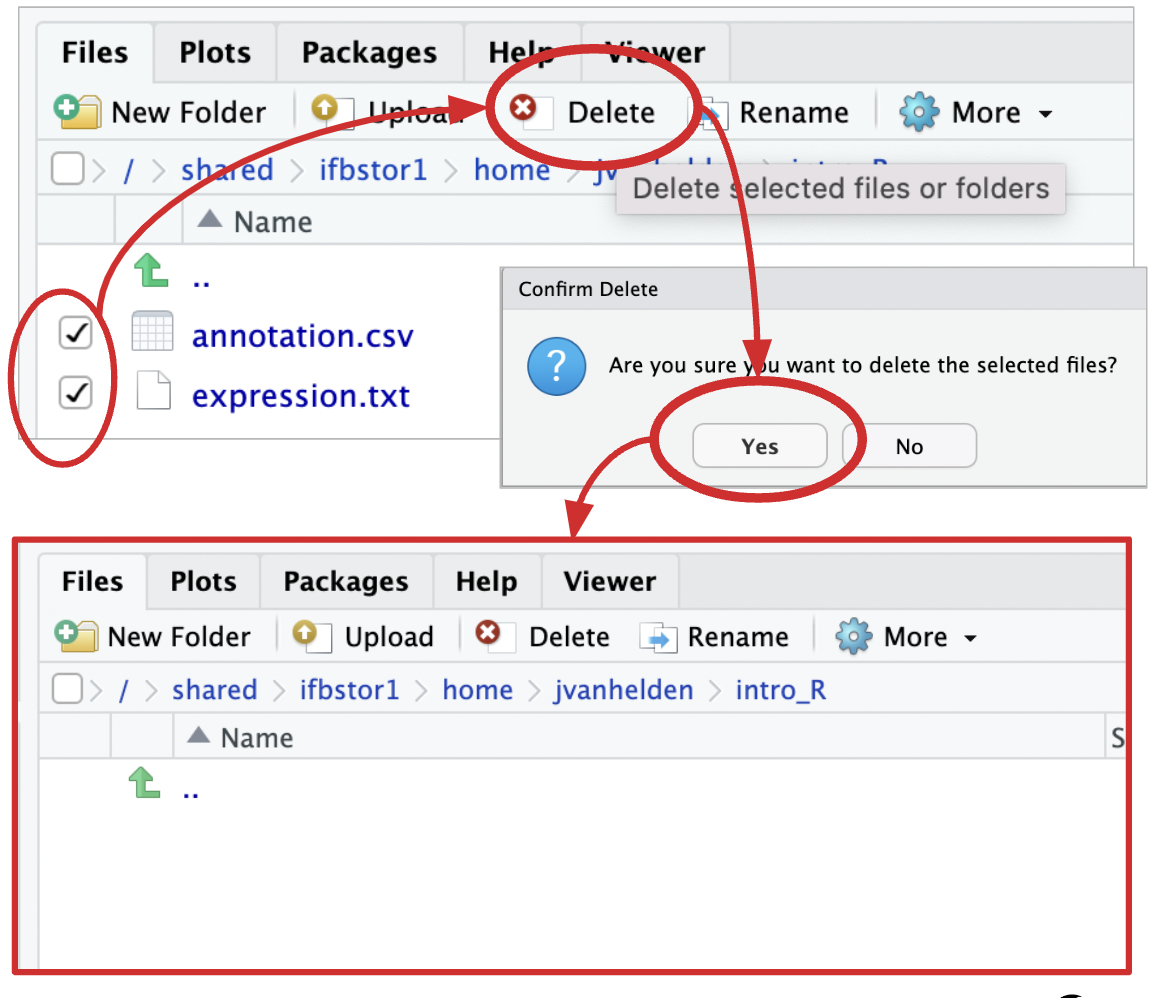
\includegraphics{images/delete.png}

Nous allons vous montrer une dernière façon de les téléverser.

\hypertarget{the-bash-geek-way-v3-directement-de-votre-home-du-cluster}{%
\section{The ``bash geek'' way (V3, directement de votre home du cluster)}\label{the-bash-geek-way-v3-directement-de-votre-home-du-cluster}}

Objectif

Dans le terminal du cluster, téléchargez et enregistrez dans votre home les fichiers de données:
- expression.txt: données d'expressions pour 4 échantillons
- annotation.csv: informations sur les gènes (id, name, chr, start, stop)

Ouvrez un connection ssh

\begin{Shaded}
\begin{Highlighting}[]
\FunctionTok{ssh}\NormalTok{ [votre\_login]@core.cluster.france{-}bioinformatique.fr}
\end{Highlighting}
\end{Shaded}

Où suis-je ?

\begin{Shaded}
\begin{Highlighting}[]
\BuiltInTok{pwd}
\end{Highlighting}
\end{Shaded}

\begin{verbatim}
## /shared/ifbstor1/projects/form_2022_32/EBAII_IntroR
\end{verbatim}

Créez un répertoire ``intro\_R''

\begin{Shaded}
\begin{Highlighting}[]
\FunctionTok{mkdir} \AttributeTok{{-}p}\NormalTok{ /shared/ifbstor1/projects/form\_2022\_32/EBAII\_IntroR/intro\_R}
\end{Highlighting}
\end{Shaded}

Déplacez-vous dans votre dossier

\begin{Shaded}
\begin{Highlighting}[]
\BuiltInTok{cd}\NormalTok{ /shared/ifbstor1/projects/form\_2022\_32/EBAII\_IntroR/intro\_R}
\end{Highlighting}
\end{Shaded}

Où suis-je maintenant ?

\begin{Shaded}
\begin{Highlighting}[]
\BuiltInTok{pwd}
\end{Highlighting}
\end{Shaded}

\begin{verbatim}
## /shared/ifbstor1/projects/form_2022_32/EBAII_IntroR
\end{verbatim}

Téléchargez les données

\begin{Shaded}
\begin{Highlighting}[]
\FunctionTok{wget}\NormalTok{ https://raw.githubusercontent.com/IFB{-}ElixirFr/EBAII/master/2022/ebaiin1/intro\_R/expression.txt }\AttributeTok{{-}{-}output{-}document}\OperatorTok{=}\NormalTok{expression.txt}
\end{Highlighting}
\end{Shaded}

\begin{verbatim}
## --2022-11-15 10:47:03--  https://raw.githubusercontent.com/IFB-ElixirFr/EBAII/master/2022/ebaiin1/intro_R/expression.txt
## Resolving raw.githubusercontent.com (raw.githubusercontent.com)... 185.199.110.133, 185.199.108.133, 185.199.111.133, ...
## Connecting to raw.githubusercontent.com (raw.githubusercontent.com)|185.199.110.133|:443... connected.
## HTTP request sent, awaiting response... 200 OK
## Length: 1747 (1.7K) [text/plain]
## Saving to: ‘expression.txt’
## 
##      0K .                                                     100% 15.8M=0s
## 
## 2022-11-15 10:47:03 (15.8 MB/s) - ‘expression.txt’ saved [1747/1747]
\end{verbatim}

\begin{Shaded}
\begin{Highlighting}[]
\FunctionTok{wget}\NormalTok{ https://raw.githubusercontent.com/IFB{-}ElixirFr/EBAII/master/2022/ebaiin1/intro\_R/annotation.csv }\AttributeTok{{-}O}\NormalTok{ annotation.csv}
\end{Highlighting}
\end{Shaded}

\begin{verbatim}
## --2022-11-15 10:47:04--  https://raw.githubusercontent.com/IFB-ElixirFr/EBAII/master/2022/ebaiin1/intro_R/annotation.csv
## Resolving raw.githubusercontent.com (raw.githubusercontent.com)... 185.199.111.133, 185.199.109.133, 185.199.108.133, ...
## Connecting to raw.githubusercontent.com (raw.githubusercontent.com)|185.199.111.133|:443... connected.
## HTTP request sent, awaiting response... 200 OK
## Length: 2326 (2.3K) [text/plain]
## Saving to: ‘annotation.csv’
## 
##      0K ..                                                    100% 25.8M=0s
## 
## 2022-11-15 10:47:04 (25.8 MB/s) - ‘annotation.csv’ saved [2326/2326]
\end{verbatim}

Qu'y a-t-il ici ?

\begin{Shaded}
\begin{Highlighting}[]
\FunctionTok{ls} \AttributeTok{{-}l}
\end{Highlighting}
\end{Shaded}

\begin{verbatim}
## total 116
## -rw-r--r--+ 1 tdenecker tdenecker  1843 Nov 15 09:19 01-intro.Rmd
## -rw-r--r--+ 1 tdenecker tdenecker   996 Nov 15 09:40 02-how.Rmd
## -rw-r--r--+ 1 tdenecker tdenecker  1478 Nov 15 09:48 03-firstSteps.Rmd
## -rw-r--r--+ 1 tdenecker tdenecker  5467 Nov 15 10:30 04-uploadData.Rmd
## -rw-r--r--+ 1 tdenecker tdenecker  1790 Nov 15 10:46 05-readData.Rmd
## -rw-r--r--+ 1 tdenecker tdenecker  1255 Nov 14 21:51 06-manipulate.Rmd
## -rw-r--r--+ 1 tdenecker tdenecker    54 Nov 14 21:51 07-references.Rmd
## -rw-rw----+ 1 tdenecker tdenecker  2326 Nov 15 10:47 annotation.csv
## -rw-r--r--+ 1 tdenecker tdenecker   267 Nov 14 21:51 book.bib
## drwxrwx---+ 2 tdenecker tdenecker  4096 Nov 15 10:47 _bookdown_files
## -rw-r--r--+ 1 tdenecker tdenecker   113 Nov 15 10:39 _bookdown.yml
## drwxrwx---+ 5 tdenecker tdenecker  4096 Nov 15 10:47 docs
## -rw-rw----+ 1 tdenecker tdenecker   247 Nov 15 09:00 EBAII_IntroR.Rproj
## -rw-rw----+ 1 tdenecker tdenecker  1747 Nov 15 10:47 expression.txt
## drwxrwx---+ 2 tdenecker tdenecker  4096 Nov 15 10:46 images
## -rw-r--r--+ 1 tdenecker tdenecker  1348 Nov 15 10:40 index.Rmd
## drwxrwx---+ 2 tdenecker tdenecker  4096 Nov 15 10:25 intro_R
## -rw-rw----+ 1 tdenecker tdenecker  1551 Nov 14 21:50 LICENSE
## drwxrwx---+ 4 tdenecker tdenecker  4096 Nov 15 10:47 _main_files
## -rw-r--r--+ 1 tdenecker tdenecker 14521 Nov 15 10:47 _main.Rmd
## -rw-r--r--+ 1 tdenecker tdenecker   500 Nov 14 21:52 _output.yml
## -rw-rw----+ 1 tdenecker tdenecker  2655 Nov 15 10:47 packages.bib
## -rw-r--r--+ 1 tdenecker tdenecker    22 Nov 14 21:51 preamble.tex
## -rw-r--r--+ 1 tdenecker tdenecker   311 Nov 15 09:29 README.md
## -rw-r--r--+ 1 tdenecker tdenecker   172 Nov 14 21:51 style.css
\end{verbatim}

A quoi ressemblent ces fichiers ?

\begin{Shaded}
\begin{Highlighting}[]
\FunctionTok{head}\NormalTok{ expression.txt}
\end{Highlighting}
\end{Shaded}

\begin{verbatim}
## id   WT1 WT2 KO1 KO2
## ENSG00000034510  235960  94264   202381  91336
## ENSG00000064201  116 71  64  56
## ENSG00000065717  118 174 124 182
## ENSG00000099958  450 655 301 472
## ENSG00000104164  4736    5019    4845    4934
## ENSG00000104783  9002    8623    7720    7142
## ENSG00000105229  1295    2744    1113    2887
## ENSG00000105723  3353    7449    3589    7202
## ENSG00000116199  2044    4525    2604    4902
\end{verbatim}

\begin{Shaded}
\begin{Highlighting}[]
\FunctionTok{head}\NormalTok{ annotation.csv}
\end{Highlighting}
\end{Shaded}

\begin{verbatim}
## id;name;chr;start;stop;strand
## ENSG00000225630;MTND2P28;1;629640;630683;+
## ENSG00000134198;TSPAN2;1;115048011;115089500;-
## ENSG00000116199;FAM20B;1;179025804;179076562;+
## ENSG00000119285;HEATR1;1;236549005;236604504;-
## ENSG00000034510;TMSB10;2;84905625;84906675;+
## ENSG00000198586;TLK1;2;170990823;171231314;-
## ENSG00000157036;EXOG;3;38496127;38542161;+
## ENSG00000157869;RAB28;4;13361354;13484365;-
## ENSG00000250202;RP11-397E7.2;4;86876338;86876652;+
\end{verbatim}

\hypertarget{actualisation-du-dossier}{%
\section{Actualisation du dossier}\label{actualisation-du-dossier}}

Dans certains cas, il faut actualiser le contenu du dossier pour pouvoir voir le nouveau sous-dossier.
Vérifiez ensuite si \texttt{intro\_R} apparaît bien dans le contenu de votre dossier principal.

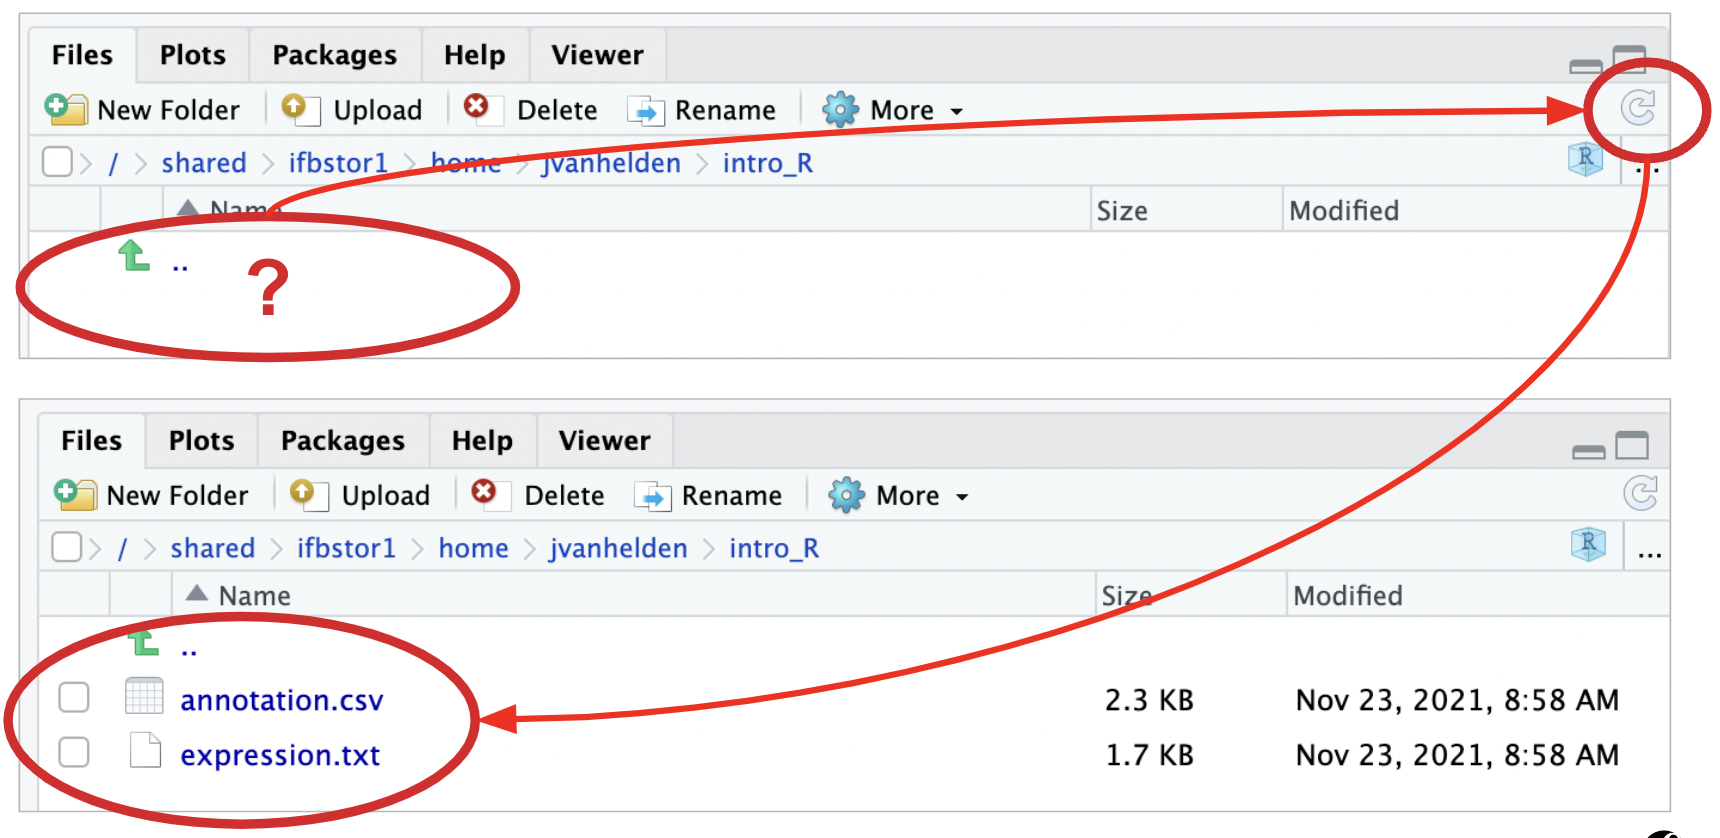
\includegraphics{images/actualiser.png}

\hypertarget{lecture-des-donnuxe9es}{%
\chapter{Lecture des données}\label{lecture-des-donnuxe9es}}

\hypertarget{chargement-des-donnuxe9es-dans-la-muxe9moire-de-r}{%
\section{Chargement des données (dans la mémoire de R)}\label{chargement-des-donnuxe9es-dans-la-muxe9moire-de-r}}

Charger le contenu du fichier ``expression.txt'' dans une variable nommée ``exprs''.

\begin{Shaded}
\begin{Highlighting}[]
\NormalTok{exprs }\OtherTok{\textless{}{-}} \FunctionTok{read.table}\NormalTok{(}\AttributeTok{file =} \StringTok{"expression.txt"}\NormalTok{, }\AttributeTok{header =} \ConstantTok{TRUE}\NormalTok{, }\AttributeTok{sep =} \StringTok{"}\SpecialCharTok{\textbackslash{}t}\StringTok{"}\NormalTok{)}
\end{Highlighting}
\end{Shaded}

Accéder à l'aide d'une fonction

\begin{Shaded}
\begin{Highlighting}[]
\FunctionTok{help}\NormalTok{(read.table)}
\end{Highlighting}
\end{Shaded}

Notation alternative

\begin{Shaded}
\begin{Highlighting}[]
\NormalTok{?read.table}
\end{Highlighting}
\end{Shaded}

Recherche interactive sous RStudio
- Sélectionner l'onglet ``Help'' du panneau inférieur droit.
- Taper ``read.table'' dans la boîte de recherche.

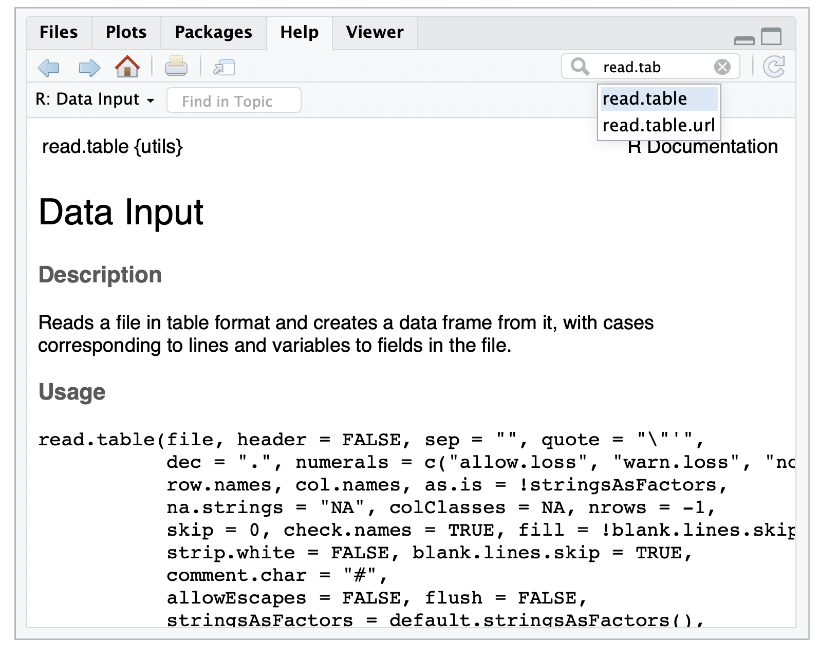
\includegraphics{images/help.png}

Sinon, une approche plus simple et plus pratique :
- demande à Google ``Comment lire une table en R ?''
- adapte l'exemple

\hypertarget{affichage-de-lobjet-exprs}{%
\section{Affichage de l'objet ``exprs''}\label{affichage-de-lobjet-exprs}}

Imprimer toutes les valeurs.

\begin{Shaded}
\begin{Highlighting}[]
\FunctionTok{print}\NormalTok{(exprs)}
\end{Highlighting}
\end{Shaded}

\begin{verbatim}
##                 id    WT1   WT2    KO1   KO2
## 1  ENSG00000034510 235960 94264 202381 91336
## 2  ENSG00000064201    116    71     64    56
## 3  ENSG00000065717    118   174    124   182
## 4  ENSG00000099958    450   655    301   472
## 5  ENSG00000104164   4736  5019   4845  4934
## 6  ENSG00000104783   9002  8623   7720  7142
## 7  ENSG00000105229   1295  2744   1113  2887
## 8  ENSG00000105723   3353  7449   3589  7202
## 9  ENSG00000116199   2044  4525   2604  4902
## 10 ENSG00000118939   7022  2526   6269  3068
## 11 ENSG00000119285  15783 17359  18591 20077
## 12 ENSG00000121680   3133  2775   2045  2796
## 13 ENSG00000125384   1380  3079    869  2419
## 14 ENSG00000129562  12089  7958  10708  7683
## 15 ENSG00000129932   1744  2247   1513  3104
## 16 ENSG00000134198    122    66     44    16
## 17 ENSG00000135452    635   427    662   291
## 18 ENSG00000140416     83   246    136   267
## 19 ENSG00000147274  16013 17642  15055 18804
## 20 ENSG00000148090    552  1062    615  1082
## 21 ENSG00000148248  62324 33973  56862 37710
## 22 ENSG00000157036   1225  1475   1275  1373
## 23 ENSG00000157869   1201  1034   1025   858
## 24 ENSG00000159433     31   788     30   675
## 25 ENSG00000161692    695  1825    746  1851
## 26 ENSG00000167005  26866 23111  24888 22661
## 27 ENSG00000168517    273   112    190    77
## 28 ENSG00000169570    202   181    207   209
## 29 ENSG00000172216   3515  1981   3204  3174
## 30 ENSG00000175221   1988  4788   2115  5306
## 31 ENSG00000183161   2238   974   2089   996
## 32 ENSG00000185324   1236  2163   1048  2024
## 33 ENSG00000188985   3415  1703   3587  2096
## 34 ENSG00000196867    209   189    293   192
## 35 ENSG00000197081  14741 36309  14941 29645
## 36 ENSG00000198586   1216  4545   1660  3932
## 37 ENSG00000214121   4044  2575   3019  2506
## 38 ENSG00000225630   1405  8135   1569  7866
## 39 ENSG00000226742    158    94    153   178
## 40 ENSG00000238241     90    43    122   143
## 41 ENSG00000248751    518   718    411   597
## 42 ENSG00000250202    261   163    177   191
## 43 ENSG00000251106     94   114     63    86
## 44 ENSG00000253991     77    78    134    92
## 45 ENSG00000254470   3025  3707   2558  4066
## 46 ENSG00000262814  15470 11450  11656 13821
## 47 ENSG00000267228   3801  2465   2787  2301
## 48 ENSG00000267699   1488  1086   1374   939
## 49 ENSG00000269293    424   162    310   120
## 50 ENSG00000279329     55    76     58    70
\end{verbatim}

Affichage des premières lignes de l'objet

\begin{Shaded}
\begin{Highlighting}[]
\FunctionTok{head}\NormalTok{(exprs)}
\end{Highlighting}
\end{Shaded}

\begin{verbatim}
##                id    WT1   WT2    KO1   KO2
## 1 ENSG00000034510 235960 94264 202381 91336
## 2 ENSG00000064201    116    71     64    56
## 3 ENSG00000065717    118   174    124   182
## 4 ENSG00000099958    450   655    301   472
## 5 ENSG00000104164   4736  5019   4845  4934
## 6 ENSG00000104783   9002  8623   7720  7142
\end{verbatim}

Affichage des dernières lignes de l'objet

\begin{Shaded}
\begin{Highlighting}[]
\FunctionTok{tail}\NormalTok{(exprs)}
\end{Highlighting}
\end{Shaded}

\begin{verbatim}
##                 id   WT1   WT2   KO1   KO2
## 45 ENSG00000254470  3025  3707  2558  4066
## 46 ENSG00000262814 15470 11450 11656 13821
## 47 ENSG00000267228  3801  2465  2787  2301
## 48 ENSG00000267699  1488  1086  1374   939
## 49 ENSG00000269293   424   162   310   120
## 50 ENSG00000279329    55    76    58    70
\end{verbatim}

Un peu plus de lignes

\begin{Shaded}
\begin{Highlighting}[]
\FunctionTok{head}\NormalTok{(exprs, }\AttributeTok{n =} \DecValTok{15}\NormalTok{)}
\end{Highlighting}
\end{Shaded}

\begin{verbatim}
##                 id    WT1   WT2    KO1   KO2
## 1  ENSG00000034510 235960 94264 202381 91336
## 2  ENSG00000064201    116    71     64    56
## 3  ENSG00000065717    118   174    124   182
## 4  ENSG00000099958    450   655    301   472
## 5  ENSG00000104164   4736  5019   4845  4934
## 6  ENSG00000104783   9002  8623   7720  7142
## 7  ENSG00000105229   1295  2744   1113  2887
## 8  ENSG00000105723   3353  7449   3589  7202
## 9  ENSG00000116199   2044  4525   2604  4902
## 10 ENSG00000118939   7022  2526   6269  3068
## 11 ENSG00000119285  15783 17359  18591 20077
## 12 ENSG00000121680   3133  2775   2045  2796
## 13 ENSG00000125384   1380  3079    869  2419
## 14 ENSG00000129562  12089  7958  10708  7683
## 15 ENSG00000129932   1744  2247   1513  3104
\end{verbatim}

Explorer le tableau dans un panneau de visualisation

\begin{Shaded}
\begin{Highlighting}[]
\FunctionTok{View}\NormalTok{(exprs)}
\end{Highlighting}
\end{Shaded}

\textbf{Note}: vous pouvez cliquer sur une en-tête de colonne pour trier les données

Explorer le tableau avec le package \href{https://rstudio.github.io/DT/}{DT}

\begin{Shaded}
\begin{Highlighting}[]
\FunctionTok{library}\NormalTok{(DT)}
\FunctionTok{datatable}\NormalTok{(exprs)}
\end{Highlighting}
\end{Shaded}

\begin{verbatim}
## PhantomJS not found. You can install it with webshot::install_phantomjs(). If it is installed, please make sure the phantomjs executable can be found via the PATH variable.
\end{verbatim}

\hypertarget{caractuxe9ristiques-dun-tableau-de-donnuxe9es}{%
\section{Caractéristiques d'un tableau de données}\label{caractuxe9ristiques-dun-tableau-de-donnuxe9es}}

\hypertarget{dimensions}{%
\subsection{Dimensions}\label{dimensions}}

Nombre de colonnes

\begin{Shaded}
\begin{Highlighting}[]
\FunctionTok{ncol}\NormalTok{(exprs)}
\end{Highlighting}
\end{Shaded}

\begin{verbatim}
## [1] 5
\end{verbatim}

Nombre de lignes

\begin{Shaded}
\begin{Highlighting}[]
\FunctionTok{nrow}\NormalTok{(exprs) }
\end{Highlighting}
\end{Shaded}

\begin{verbatim}
## [1] 50
\end{verbatim}

Dimensions

\begin{Shaded}
\begin{Highlighting}[]
\FunctionTok{dim}\NormalTok{(exprs)}
\end{Highlighting}
\end{Shaded}

\begin{verbatim}
## [1] 50  5
\end{verbatim}

\hypertarget{noms-des-colonnes-et-des-lignes}{%
\subsection{Noms des colonnes et des lignes}\label{noms-des-colonnes-et-des-lignes}}

Noms des colonnes

\begin{Shaded}
\begin{Highlighting}[]
\FunctionTok{colnames}\NormalTok{(exprs)}
\end{Highlighting}
\end{Shaded}

\begin{verbatim}
## [1] "id"  "WT1" "WT2" "KO1" "KO2"
\end{verbatim}

Idem

\begin{Shaded}
\begin{Highlighting}[]
\FunctionTok{names}\NormalTok{(exprs) }
\end{Highlighting}
\end{Shaded}

\begin{verbatim}
## [1] "id"  "WT1" "WT2" "KO1" "KO2"
\end{verbatim}

Noms des lignes

\begin{Shaded}
\begin{Highlighting}[]
\FunctionTok{rownames}\NormalTok{(exprs)}
\end{Highlighting}
\end{Shaded}

\begin{verbatim}
##  [1] "1"  "2"  "3"  "4"  "5"  "6"  "7"  "8"  "9"  "10" "11" "12" "13" "14" "15"
## [16] "16" "17" "18" "19" "20" "21" "22" "23" "24" "25" "26" "27" "28" "29" "30"
## [31] "31" "32" "33" "34" "35" "36" "37" "38" "39" "40" "41" "42" "43" "44" "45"
## [46] "46" "47" "48" "49" "50"
\end{verbatim}

\hypertarget{ruxe9sumuxe9-rapide-des-donnuxe9es-par-colonne}{%
\subsection{Résumé rapide des données par colonne}\label{ruxe9sumuxe9-rapide-des-donnuxe9es-par-colonne}}

Statistiques par colonne

\begin{Shaded}
\begin{Highlighting}[]
\FunctionTok{summary}\NormalTok{(exprs)}
\end{Highlighting}
\end{Shaded}

\begin{verbatim}
##       id                 WT1              WT2               KO1          
##  Length:50          Min.   :    31   Min.   :   43.0   Min.   :    30.0  
##  Class :character   1st Qu.:   264   1st Qu.:  203.2   1st Qu.:   228.5  
##  Mode  :character   Median :  1338   Median : 1903.0   Median :  1324.5  
##                     Mean   :  9358   Mean   : 6498.6   Mean   :  8356.0  
##                     3rd Qu.:  3730   3rd Qu.: 4727.2   3rd Qu.:  3491.2  
##                     Max.   :235960   Max.   :94264.0   Max.   :202381.0  
##       KO2         
##  Min.   :   16.0  
##  1st Qu.:  223.5  
##  Median : 2060.0  
##  Mean   : 6489.5  
##  3rd Qu.: 4926.0  
##  Max.   :91336.0
\end{verbatim}

Structure de la variable

\begin{Shaded}
\begin{Highlighting}[]
\FunctionTok{str}\NormalTok{(exprs)}
\end{Highlighting}
\end{Shaded}

\begin{verbatim}
## 'data.frame':    50 obs. of  5 variables:
##  $ id : chr  "ENSG00000034510" "ENSG00000064201" "ENSG00000065717" "ENSG00000099958" ...
##  $ WT1: int  235960 116 118 450 4736 9002 1295 3353 2044 7022 ...
##  $ WT2: int  94264 71 174 655 5019 8623 2744 7449 4525 2526 ...
##  $ KO1: int  202381 64 124 301 4845 7720 1113 3589 2604 6269 ...
##  $ KO2: int  91336 56 182 472 4934 7142 2887 7202 4902 3068 ...
\end{verbatim}

Même résultat que dans le panneau ``Environment''

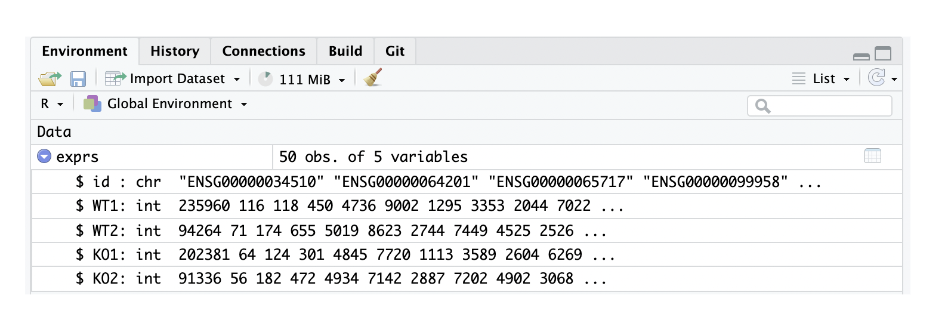
\includegraphics{images/envExpr.png}

\hypertarget{sharing-your-book}{%
\chapter{Sharing your book}\label{sharing-your-book}}

\hypertarget{publishing}{%
\section{Publishing}\label{publishing}}

HTML books can be published online, see: \url{https://bookdown.org/yihui/bookdown/publishing.html}

\hypertarget{pages}{%
\section{404 pages}\label{pages}}

By default, users will be directed to a 404 page if they try to access a webpage that cannot be found. If you'd like to customize your 404 page instead of using the default, you may add either a \texttt{\_404.Rmd} or \texttt{\_404.md} file to your project root and use code and/or Markdown syntax.

\hypertarget{metadata-for-sharing}{%
\section{Metadata for sharing}\label{metadata-for-sharing}}

Bookdown HTML books will provide HTML metadata for social sharing on platforms like Twitter, Facebook, and LinkedIn, using information you provide in the \texttt{index.Rmd} YAML. To setup, set the \texttt{url} for your book and the path to your \texttt{cover-image} file. Your book's \texttt{title} and \texttt{description} are also used.

This \texttt{gitbook} uses the same social sharing data across all chapters in your book- all links shared will look the same.

Specify your book's source repository on GitHub using the \texttt{edit} key under the configuration options in the \texttt{\_output.yml} file, which allows users to suggest an edit by linking to a chapter's source file.

Read more about the features of this output format here:

\url{https://pkgs.rstudio.com/bookdown/reference/gitbook.html}

Or use:

\begin{Shaded}
\begin{Highlighting}[]
\NormalTok{?bookdown}\SpecialCharTok{::}\NormalTok{gitbook}
\end{Highlighting}
\end{Shaded}


  \bibliography{book.bib,packages.bib}

\end{document}
